% !TeX spellcheck = de_DE
%\documentclass[11pt,a4paper]{article}
\documentclass[11pt
  , a4paper
  , article
  , oneside
%  , twoside
%  , draft
]{memoir}

\usepackage{control}
\usepackage[numbers]{natbib}


\begin{document}

\newcommand{\technumber}{
  RAON Control-Document Series\\
  Revision : v1.0,   Release : 2014-12-24 fixed date}
\title{\textbf{Archiver Appliance 구성}}

\author{이상일\thanks{silee7103@ibs.re.kr} \\

  Rare Isotope Science Project\\
  Institute for Basic Science, Daejeon, South Korea
}
\date{\today}

\renewcommand{\maketitlehooka}{\begin{flushright}\textsf{\technumber}\end{flushright}}
%\renewcommand{\maketitlehookb}{\centering\textsf{\subtitle}}
%\renewcommand{\maketitlehookc}{C}
%\renewcommand{\maketitlehookd}{D}

\maketitle

\begin{abstract}
RAON control system uses the EPICS middle ware as the software framework of the control system. The every local machines of the RAON will be integrated based on the EPICS framework. The method of the data storing based on the EPICS framework is classified in three ways largely. One is the classic channel archiver of the file-based approach, another is the channel archiver using the relational database approach and the other is the archive appliance complementing the disadvantages of the first and the second approach. The problem of the first mentioned approach, "classic channel archiver", has been being related to the index file of the meta-data indexing the real data block. That of the second mentioned approach, "relational database channel archiver", has been being issued about the performance of the file I/O. In recent, the solution, "archiver appliance", compensating for these problems was developed by the Stanford Linear Accelerator Center (SLAC) national laboratory of the United States.

This paper describes how to build-up the two or more archive appliances on the data storage to be applied the test facility of the cryogenic control system and evaluates the performance and the reliability of those in detail.
\end{abstract}

EPICS framework\cite{epics}의 CA(Channel Access) 프로토콜을 통한 PV(Process Variable)의 값에 대한 데이터 저장은 크게 세 가지 형태의 확장 utility가 사용된다. 하나는 현재 단계에서 classic channel archiver로 불리는 파일 형태로 데이터를 저장하는 Channel Archiver\cite{archiver} 이며, 다른 하나는 RDBMS(Relational Database Management System)을 사용하는 RDB Archiver\cite{rdbarchiver} 이며, 마지막 하나는 본 문서에서 설명하려는 Archver Appliance 이다. Archiver Appliance\cite{appliance}는 SLAC(Stanford Linear Accelerator Center)의 National Laboratory에서 개발된 EPICS Data 저장용 utility 이다. Archiver Appliance\cite{appliance}는 네가지의 모듈로 구성된다. Engine, Retrieval, ETL(Extraction, Transformation and Load) 그리고 Management(MGMT) 모듈로 구성된다. 본 문서에서는 기존의 두 데이터 저장 utility의 특성 및 이슈 사항을 살펴보고, 그에 대한 문제점을 보완하여 개발된 Archiver Appliance의 특성, 모듈 구성, 설정 방법 및 데이터 저장영역에 따른 file I/O 성능 분석에 대하여 기술한다. 각 세 가지 utility에 대한 특성을 살펴보면 아래와 같다.


\hfil\break
\chapter{Channel Archiver}
\section{특성}
Channel Archiver\cite{archiver}는 초기 EPICS CA 프로토콜의 PV 데이터를 저장하는 EPICS extension utilities 중 하나로 개발 되었으며 다년간 EPICS community에서 활발하게 사용된 어플리케이션이다. 기본 구성은 PV 데이터에 대한 데이터 블럭(일종의 meta data)의 정보를 담고 있는 index file이 존재하며 해당 index 파일의 정보를 통하여 데이터 블럭에 접근하여 데이터를 획득한다. 파일 I/O에 대한 성능은 60,000 samples/sec을 보이며, RDB Archiver에 비해 높은 성능을 보이지만 여전히 대용량 데이터를 저장하기 위한 구조에는 개선의 여지가 있으며 현재 Channel Archiver에 대한 개발은 더이상 진행되지 않는 상태이다.
\section{이슈 사항}
Channel Archiver\cite{archiver}는 구조적으로 index 파일을 사용한다. 이 경우 저장을 위한 PV list가 많거나 sampling rate이 높은 PV가 오랜시간 데이터를 저장할 경우 index 파일의 크기가 2GByte를 초과 할 경우 index 파일을 조작하는 모듈에 성능 부하가 발생하여 데이터 저장 성능이 급속히 떨어진다. 또한, 해당 시스템의 임의적인 재부팅, 또는 Archive Engine의 이상으로 Engine을 강제 종료시 특정 데이터 블럭과 index 파일간의 mismatch가 발생하며 그 경우 해당 데이터의 블럭을 읽을 수 없게 되는 문제점 등이 있다.
\begin{itemize}
	\item Index file의 크기 (2GByte 초과시 파일 입출력 성능 저하)
	\item Index file과 Data block간의 mismatch
\end{itemize}
\hfil\break

\chapter{RDB Archiver}
\section{특성}
Oracle, MySQL, PostgreSQL등의 RDMBS를 이용하여 구현된 RDB Archiver\cite{rdbarchiver}는 기존 classic channel archiver에서 가지는 index file의 제약사항에서 벗어날 수 있게 되었으며, 범용적으로 사용되는 SQL 쿼리 문을 통해 사용자가 데이터를 자유롭게 추출해 낼 수 있어 client 프로그램 개발에 많은 자유도를 부여 할 수 있게 되었다.

\section{이슈 사항}
Index 파일 제약사항의 해결과 SQL 사용의 편리함에도 불구하고 DBMS가 가지고 있는 한계로 사용에 많은 제약사항이 발생하였다. DBMS는 구조적으로 작은 transaction 단위로 사용자 쿼리문을 수행함에 있어 "all or nothing"에 초점이 맞추어져 있다. DBMS는 수행 되어야 할 쿼리 문이 transaction 단위로 모두 완료 되었거나 아니면 전혀 없었던 일로 되돌려야 하는 commit/rollback 기능을 수행하여야 한다. 이러한 구조는 내부동작 메커니즘이 매우 까다로우며, 결과적으로 RDB Archiver의 성능에 제약사항을 작용한다. 고속의 많은 scientfic data를 처리해야 하는 상황에서 파일 I/O에 대한 성능은 매우 중요시 여겨진다. RDB Archiver에 대한 이러한 이슈사항들은 EPICS commnunity에서 레포트 되어지고 있는 상황이다.
Database community 내에서도 고속의 대용량 scientific data를 처리하기 위한 움직임으로 sciDB(scientific database)\cite{scidb} 등이 연구 되어지고 있는 상황이지만 아직능지 안정적인 운전과 성능에는 많은 문제가 남아있는 상태이다.

\begin{itemize}
	\item 분산환경의 DBMS 운용의 어려움
	\item 데이터 입출력 파일 I/O의 성능이 낮음(7,000samples/sec)
\end{itemize}

\chapter{Archiver Appliance}

\section{특성}
Archiver Appliance\cite{appliance}는 상위에서 언급된 이슈사항을 모두 해결한 utiility로 점차적으로 EPICS community내에서 사용이 증가하고 있는 상태이다. 주요 특징으로는 classic channel archiver에서 문제되고 있는 index 파일을 가지는 구조를 제거 하였으며, file I/O를 극대화하기 위한 방식으로 로컬파일시스템과 메모리 맵핑되는 RAM filesystem을 사용하였다. 또한, Single Archiver Appliance를 그대로 확장하여 Multiple Archive Appliance를 구성하여 기존에 문제가 되었던 확장성을 해결하였다. 이러한 확장성은 데이터 저장 시스템을 클러스터 형태로 설계가 가능하도록 하였으며, 데이터 추출도 병렬로 처리하여 부하 분산과 데이터 추출 속도를 혁신적으로 단축 시켰다. 주요특징을 살펴보면 아래와 같다.
\begin{itemize}
	\item cluster 상에 appliance 추가 만으로 cluster appliances를 scale out
	\item ETL 모듈을 이용하여 각 스토리지 영역간의 기간별 데이터 이동
	\begin{itemize}
		\item 제한된 STS RAM filesystem 영역을 계속적으로 사용하여 성능향상 가능
		\item 스토리지 성능에 따라 계층적 데이터 저장 가능
	\end{itemize}
	\item 데이터 추출 성능 (Data read I/O) 확대
	\item A management interface giving you the ability to manage and monitor the system using a browser.
	\begin{itemize}
		\item The ability to add PVs to a cluster of appliances using a browser (perhaps by users).
		\item Various metrics to help with capacity planning.
		\item Ability to define system-wide defaults for archiving parameters using policies.
	\end{itemize}
	\item Python, Matlab 등의 외부 언어와의 Binding
	\item Ability to customize the appliance to suit a different set of requirements
	\begin{itemize}
		\item 사용자 환경에 최적화된 스토리지 시스템 구성이 가능하다.
		\item 데이터 추출 응답에 대한 새로운 Mime 형식을 쉽게 추가 가능하다.
		\end{itemize}
\end{itemize}

\section{System 요구사항}
Archiver Appliance 구성을 위하여는 아래와 같은 요구사항을 만족해야 한다.
\begin{itemize}
	\item Sun Java JDK 1.7 버전 이상, JRE가 아닌 JDK 버전이어야 한다.
	\item Tomcat 7.x 이상\cite{apachetomcat}, apache-tomcat-7.0.22 이상
	\item Management UI는 firefox나 chrome에 최적화 되어 있다.
	\item EPICS Channel Access는 CAJ(Channel Access for Java)가 번들로 포함된다.
	\item 옵션으로 설정 configuration을 DB에 저장하기 위하여 MySQL mysql-5.1 이상을 설치한다.
	\item 데이터 프로토콜은 google protocol buffer\cite{protobuffer}를 사용하므로, archiverviewer 또는 CSS의 data browser를 사용시 해당 모듈이 plug-in 되어 있는 버젼을 사용해야 한다.
\end{itemize}

\section{모듈 구성}
Archiver Appliance는 아래와 같이 4개의 모듈로 구성되며, 각 모듈은 아래 항목에서 상세히 설명한다.

\begin{itemize}
	\item Engine
	\item Retrieval
	\item ETL(Extraction, Transformation, Load)
	\item MGMT(Management)
\end{itemize}
구현 측면에서의 특성은 Archiver Appliance는 Java Channel Access를 이용한 Java 언어로 개발 되었으며, 기존 Client 툴(Archiver Viewer, Data Browser)과의 호환성을 위하여 새롭게 데이터 구조를 정의하여 각 툴의 플러그인 모듈로 제공하였다. 이때 데이터 구조에 정의하는데 사용된 것은 google에서 protocol 정의에 사용되는 google protocol buffer를 사용하였다. 여기에 추가적으로 범용적으로 사용되어지고 있는 python과의 인터페이스를 위하여 python 인터페이스 라이브러리를 추가하였다. 그림 \ref{fig:single_appliance}은 Single Archiver Appliance 구성을 보여준다. 데이터 저장영역은 STS(Short Term Storage, RAM Disk=ramfs), MTS(Medium Term Storage, SATA Disk=ext4) 및 LTS(Long Term Storage, Network=glusterfs)로 구성된다. STS 영역은 Appliance가 기동되면서 가용할 수 있는 메모리를 범주를 확인하여 메모리 영역과 파일 시스템 영역을 맵핑한 RAM disk의 ram filesystem을 생성한다. 이는 로컬 영역에서 파일 I/O 성능을 극대화하기 위한 방법으로 사용된다. MTS 영역은 일반적인 SATA disk로 구성되며, LTS 영역은 일반 ethernet 네트워크를 통하여 glusterfs로 구성할 수 있다. 좀 더 효율적인 Archiver Appliance 성능 구현을 위해서는 MTS와 LTS 영역에 대한 설계가 필요하다.
 
\begin{figure}[h!]
	\centering
	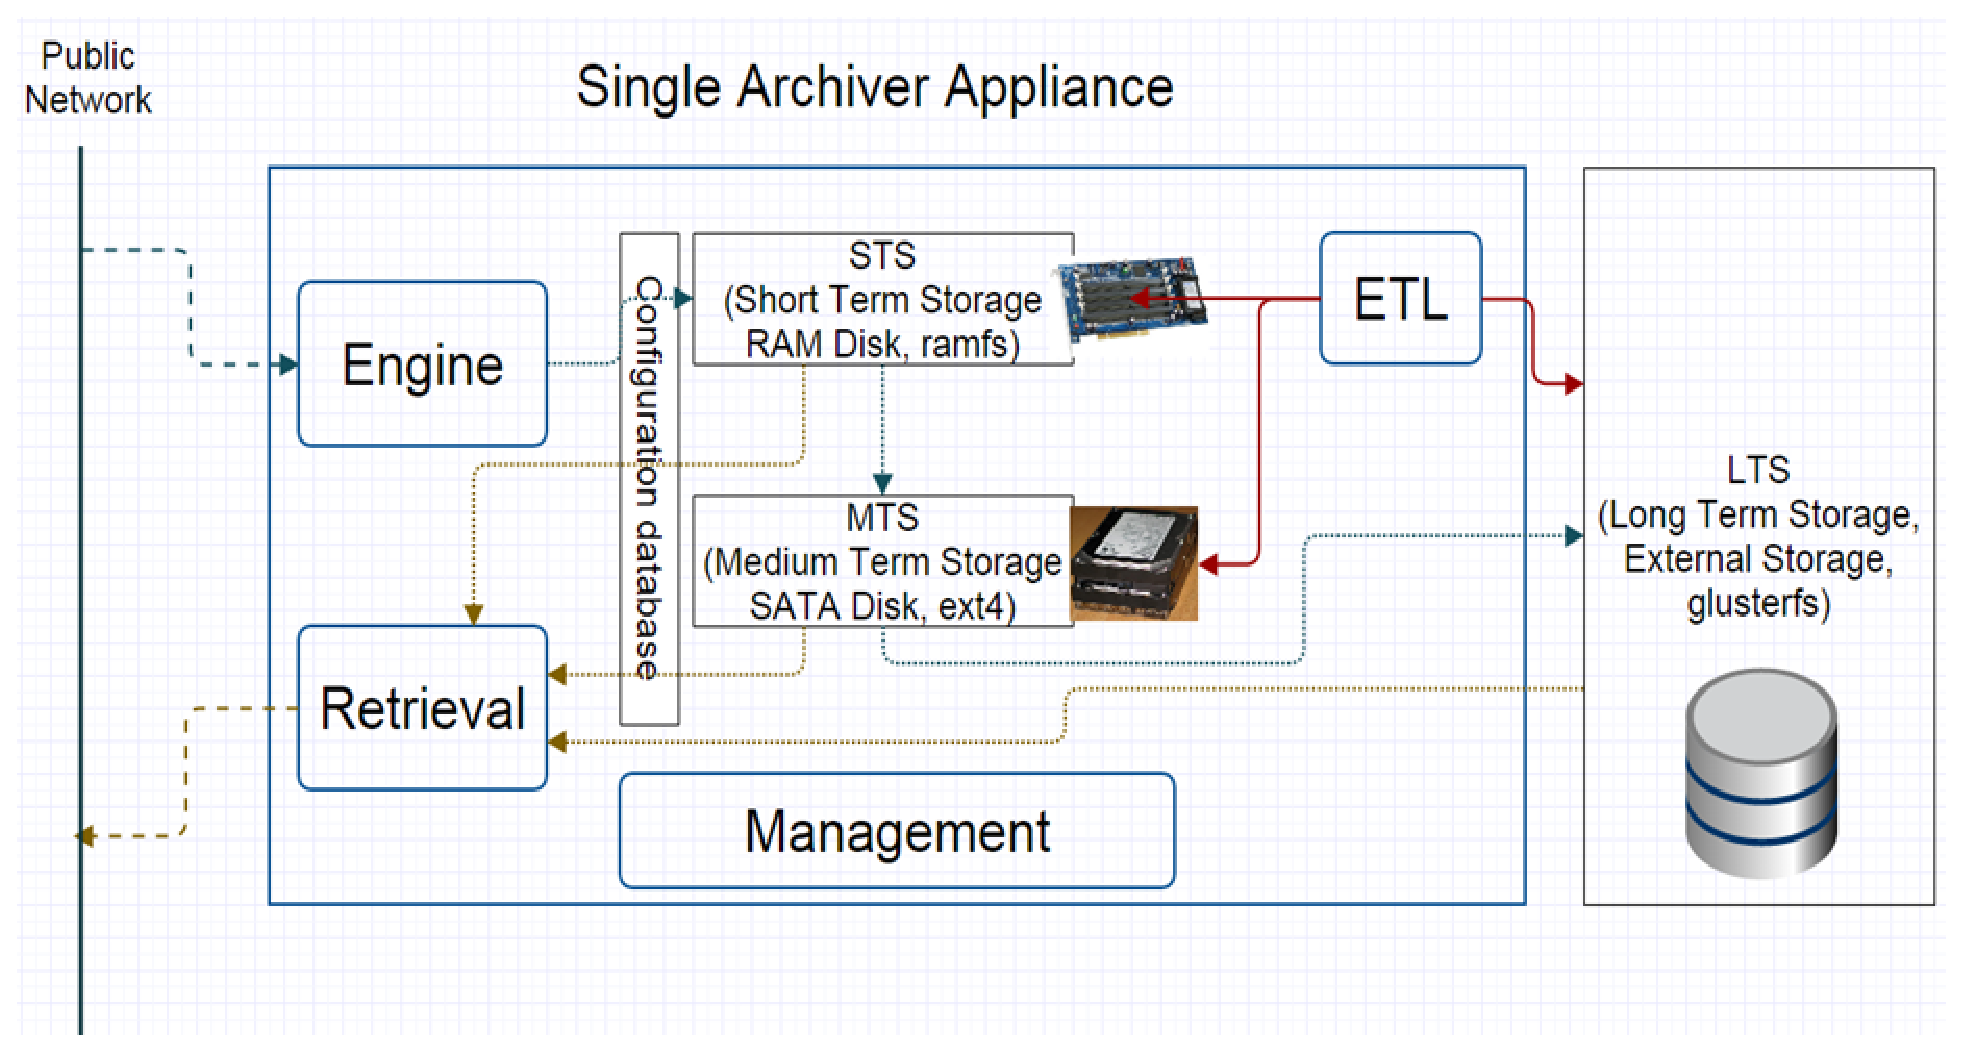
\includegraphics[width=0.85\textwidth]{./images/image-3.eps}
	\caption{Single Archiver Appliance}
	\label{fig:single_appliance} 
\end{figure}

\subsection*{Engine 모듈}
Engine 모듈은 그림 \ref{fig:single_appliance}에서와 같이 "Public Network"와 연결되어 EPICS CA 프로토콜를 통하여 획득하는 PV 데이터 값을 정의된 RAM disk의 STS 영역에 저장한다. STS 영역은 각 Appliance node가 파일 I/O의 성능을 극대화하기 위하여 자신의 메모리영역을 RAM Disk 영역으로 메모리 맵핑하여 사용하는 저장공간이다. 각 Appliance의 노드는 MGMT 모듈에서 설정된 PV list와 각 PV 저장 정책에 따라서 데이터를 저장한다. 데이터 파일정보에 대한 index file(메터 데이터)을 제거하기 위하여 저장 파일의 이름에 EPICS PV의 naming convention 및 시각 정보를 적용한다. 각 PV는 하나의 단위로 파일의 하나로 생성된며 그 사용예는 아래와 같다. 아래 예에서와 같이 PV의 Naming은 데이터 저장의 디렉토리 계층을 이룬다. 따라서 체계적인 데이터 관리를 위하여는 잘 조직화된 PV의 Naming convention의 정의가 매우 중요한 요소 중 하나이다.
\\
예) Average temperature of the 42nd RACK of SCL11(LLRF)에 대한 PV Naming \\ 
\textit{SCL11-LLRF:Rack042:TempAvg}
\begin{lstlisting}[style=termstyle]
SCL11-LLRF/
   `-- Rack042
      |-- TempAvg:2014_11_23.pb
      |-- TempAvg:2014_11_24.pb
      `-- TempAvg:2014_11_25.pb
ECR13-Mag/
   `-- PS012
      |-- CurrentRB:2014_11_23.pb
      |-- CurrentRB:2014_11_23.pb
      `-- CurrentRB:2014_11_23.pb
MEBT3-Diag/
   `-- BPM004
      |-- XRaw:2014_11_23.pb
      |-- XRaw:2014_11_23.pb
      `-- XRaw:2014_11_23.pb
Cryo-TFC/
   `-- Pmp014
      |-- PowerSetpt:2014_11_23.pb
      |-- PowerSetpt:2014_11_23.pb
      `-- PowerSetpt:2014_11_23.pb
\end{lstlisting}

\subsection*{Retrieval 모듈}
Retrieval 모듈은 그림 \ref{fig:single_appliance}에서 보면 세 가지의 스토리지 영역(STS, MTS 및 LTS)에서 데이터를 추출한다. 사용자가 요청하는 데이터 추출 날짜에 따라 세 스토리지 영역으로 부터 데이터를 추출한다. 그림 \ref{fig:python_ext}는 범용적으로 사용되는 python을 사용하여 저장된 EPICS 데이터를 추출하는 예를 보여준다. 
\hfil\break

\begin{lstlisting}[style=termstyle]
Python 2.7.3 (default, Mar 13 2014, 11:03:55) 
[GCC 4.7.2] on linux2
Type "help", "copyright", "credits" or "license" for more information.
>>> import json
>>> import urllib2
>>> retrieval='http://10.1.4.222:17665/retrieval/data/getData.json'
>>> dateresp= urllib2.urlopen(url=retrieval +  '?pv=PI222:sin:1')
>>> data = json.load(dateresp)
>>> print len(data[0]['data'])
>>> print data[0]['data'][0]
\end{lstlisting}

\begin{figure}[h!]
	\centering
	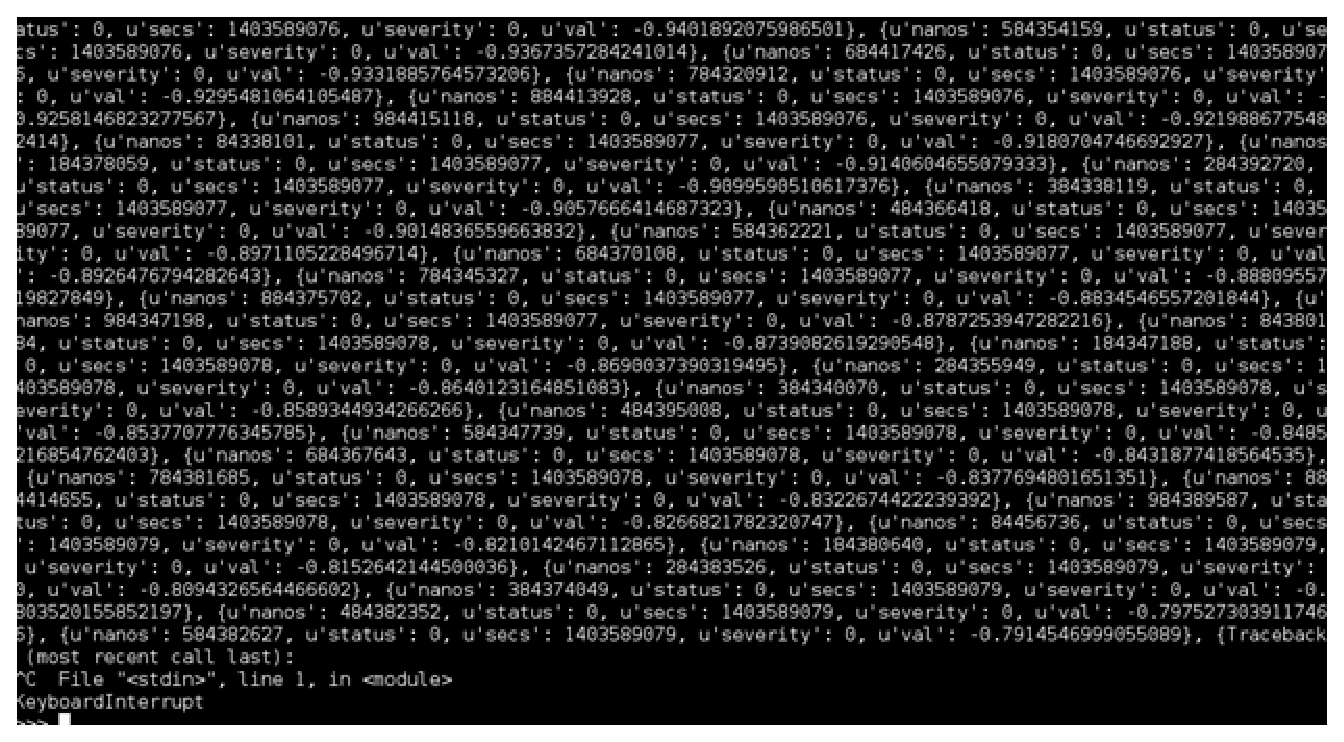
\includegraphics[width=0.85\textwidth,height=0.55\textwidth]{./images/image-7.eps}
	\caption{Python Data 추출}
	\label{fig:python_ext} 
\end{figure}


아래 그림 \ref{fig:viewer} Archiver Viewer를 통하여 데이터를 획득한 화면이다. Archiver Viewer와 Appliance의 Retrieval 모듈 간의 protocol을 google protocol buffer를 사용하여 구성 되었으며, 해당 모듈간의 데이터 interface를 위해서는 아래와 같은 프로토콜 접속을 통해 접속한다.
\begin{lstlisting}[style=termstyle]
$>java -jar archiverviewer.jar -u pbraw://appliance_ip_address:17665/retrieval
\end{lstlisting}

\begin{figure}[h!]
	\centering
	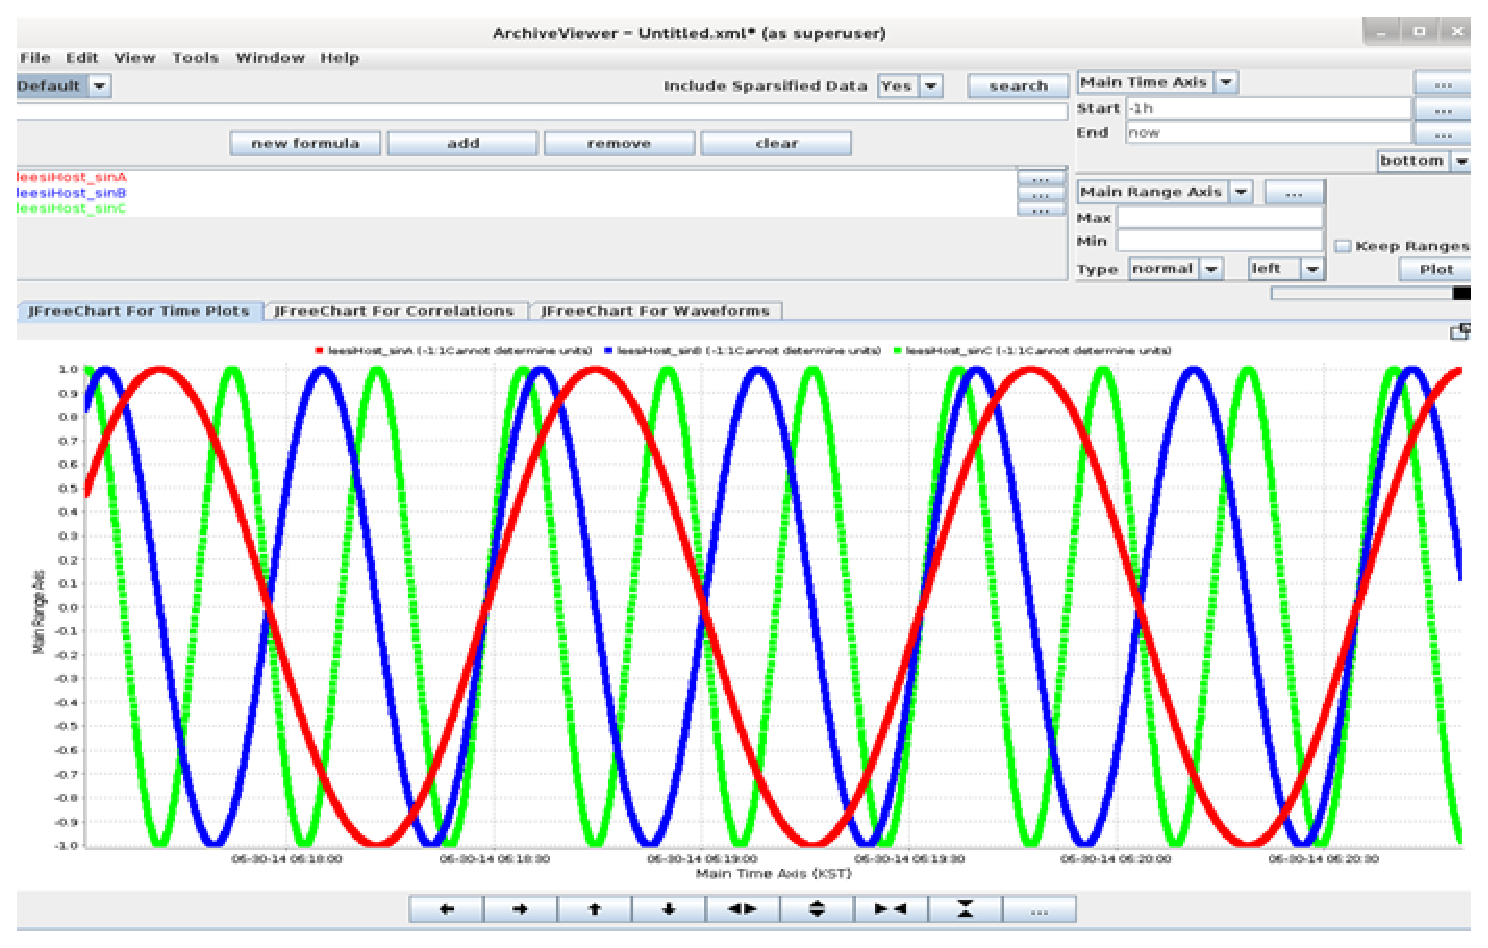
\includegraphics[width=0.85\textwidth, height=0.55\textwidth]{./images/image-6.eps}
	\caption{Archive Viewer Data 추출}
	\label{fig:viewer} 
\end{figure}

\subsection*{ETL 모듈}
Extraction, Transformation, Load 모듈은 아래 policies.py 설정에 따라 STS, MTS 및 LTS의 스토리지 영역을 지정할 수 있으며, 그에 대한 데이터 partitioning 정책을 부여 할 수 있다. 또한, 각 site의 특성에 최적화된 정책을 수정 할 수 있다. 그림 \ref{fig:single_appliance}에서 ETL 모듈은 정책에서 부여 받은 설정에 따라 STS 영역의 데이터를 MTS영역에 시간대 별로 이동하여 합성한다. 또한, MTS 영역의 데이터 역시 LTS에 설정시간에 따라 이동하여 합성한다.

\begin{lstlisting}[style=termstyle]
import sys
import os

# Generate a list of policy names. This is used to feed the dropdown in the UI.
def getPolicyList():
pvPoliciesDict = {}
pvPoliciesDict['Default'] = 'The default policy'
pvPoliciesDict['BPMS'] = 'BPMS that generate more than 1GB a yer'
pvPoliciesDict['2HzPVs'] = 'PVs with an event rate more than 2Hz'
pvPoliciesDict['3DaysMTSOnly'] = 'Store data for 3 days upto the MTS only.'
return pvPoliciesDict

# Define a list of fields that will be archived as part of every PV.
# The data for these fields will included in the stream for the PV.
# We also make an assumption that the data type for these fields is the same as that of the .VAL field

def getFieldsArchivedAsPartOfStream():
return ['HIHI','HIGH','LOW','LOLO','LOPR','HOPR','DRVH','DRVL'];


# We use the environment variables ARCHAPPL_SHORT_TERM_FOLDER and ARCHAPPL_MEDIUM_TERM_FOLDER to determine the location of the STS an
shorttermstore_plugin_url = 'pb://localhost?name=STS&rootFolder=${ARCHAPPL_SHORT_TERM_FOLDER}&partitionGranularity=PARTITION_HOUR&con
mediumtermstore_plugin_url = 'pb://localhost?name=MTS&rootFolder=${ARCHAPPL_MEDIUM_TERM_FOLDER}&partitionGranularity=PARTITION_DAY&ho
longtermstore_plugin_url = 'pb://localhost?name=LTS&rootFolder=${ARCHAPPL_LONG_TERM_FOLDER}&partitionGranularity=PARTITION_YEAR'


def determinePolicy(pvInfoDict):
pvPolicyDict = {}
    userPolicyOverride = ''
    if 'policyName' in pvInfoDict:
    userPolicyOverride = pvInfoDict['policyName']
    
    if userPolicyOverride == '2HzPVs' or (userPolicyOverride == '' and pvInfoDict['eventRate'] > 2.0):
    pvPolicyDict['samplingPeriod'] = 1.0
    pvPolicyDict['samplingMethod'] = 'MONITOR'
    pvPolicyDict['dataStores'] = [
    shorttermstore_plugin_url,
    mediumtermstore_plugin_url,
    longtermstore_plugin_url
    ]
    pvPolicyDict['policyName'] = '2HzPVs';
    elif userPolicyOverride == 'Default' or (userPolicyOverride == '' and pvInfoDict['pvName'] == 'mshankar:arch:sine'):
    pvPolicyDict['samplingPeriod'] = 1.0
    pvPolicyDict['samplingMethod'] = 'MONITOR'
    pvPolicyDict['dataStores'] = [
    shorttermstore_plugin_url,
    mediumtermstore_plugin_url,
    longtermstore_plugin_url + "&pp=firstSample&pp=firstSample_3600"
    ]
    pvPolicyDict['policyName'] = 'Default';
    elif userPolicyOverride == 'BPMS' or (userPolicyOverride == '' and pvInfoDict['pvName'].startswith('BPMS') and pvInfoDict['storag
    # We limit BPM PVs to 1GB/year (34 bytes/sec)
    # We reduce the sampling rate (and hence increase the sampling period) to cater to this. 
    pvPolicyDict['samplingPeriod'] = pvInfoDict['storageRate']/(35*pvInfoDict['eventRate'])
    pvPolicyDict['samplingMethod'] = 'MONITOR'
    pvPolicyDict['dataStores'] = [
    shorttermstore_plugin_url,
    mediumtermstore_plugin_url,
    longtermstore_plugin_url
    ]
    pvPolicyDict['policyName'] = 'BPMS';
    elif userPolicyOverride == '3DaysMTSOnly':
    pvPolicyDict['samplingPeriod'] = 1.0
    pvPolicyDict['samplingMethod'] = 'MONITOR'
    pvPolicyDict['dataStores'] = [
    shorttermstore_plugin_url,
    # We want to store 3 days worth of data in the MTS.
    'pb://localhost?name=MTS&rootFolder=${ARCHAPPL_MEDIUM_TERM_FOLDER}&partitionGranularity=PARTITION_DAY&hold=4&gather=1',
    'blackhole://localhost?name=LTS'
    ]
    pvPolicyDict['policyName'] = '2HzPVs';
    else:
    pvPolicyDict['samplingPeriod'] = 1.0
    pvPolicyDict['samplingMethod'] = 'MONITOR'
    pvPolicyDict['dataStores'] = [
    shorttermstore_plugin_url,
    mediumtermstore_plugin_url,
    longtermstore_plugin_url
    ]
    pvPolicyDict['policyName'] = 'Default';
 archiveFields=[]
            
 if "RTYP" not in pvInfoDict:
     pvPolicyDict["archiveFields"]=archiveFields
 else:
     pvRTYP=pvInfoDict["RTYP"]
     if pvRTYP=="ai":
         archiveFields=['HIHI','HIGH','LOW','LOLO','LOPR','HOPR']
     elif pvRTYP=="ao":
         archiveFields=['HIHI','HIGH','LOW','LOLO','LOPR','HOPR','DRVH','DRVL']
     elif pvRTYP=="calc":
         archiveFields=['HIHI','HIGH','LOW','LOLO','LOPR','HOPR']
     elif pvRTYP=="calcout":
         archiveFields=['HIHI','HIGH','LOW','LOLO','LOPR','HOPR']
     elif pvRTYP=="longin":
         archiveFields=['HIHI','HIGH','LOW','LOLO','LOPR','HOPR']
     elif pvRTYP=="longout":
         archiveFields=['HIHI','HIGH','LOW','LOLO','LOPR','HOPR','DRVH','DRVL']
     elif pvRTYP=="dfanout":
         archiveFields=['HIHI','HIGH','LOW','LOLO','LOPR','HOPR']
     elif pvRTYP=="sub":
         archiveFields=['HIHI','HIGH','LOW','LOLO','LOPR','HOPR']
     pvPolicyDict["archiveFields"]=archiveFields
            
  return pvPolicyDict
                
\end{lstlisting}
정책 설정파일 policies.py을 설정하는 경로는 아래와 같다.
\begin{lstlisting}[style=termstyle]
$>export ARCHAPPL_POLICIES=/archiver_appliance_directory/policies.py
\end{lstlisting}

만약, Site 특성에 따른 build를 한다면 policies.py 파일은 ARCHAPPL\_POLICIES 환경 변수에 정의된 것을 따르지 않고 그것을 대신하여 각 Site 특성에 따른 build 시 mgmt war 파일의 일부로 포함된다. 따라서 아래와 같이 환경변수가 정의 되었다면 "SITE\_SPECIFIC\_PATH/classes/" 상에 포함되게 된다.
\begin{lstlisting}[style=termstyle]
$>export ARCHAPPL_SITEID=SITE_SPECIFIC_PATH
\end{lstlisting}

\subsection*{MGMT(Management) 모듈}
MGMT 모듈은 그림 \ref{fig:mgmt_appliance}에서 보듯이 Appliance의 기동후 아래와 같은 URL 주소를 이용하여 웹브라우저 상에서 확인 가능하다. 아래 접속 통신 포트 번호는 환경 설정에 따라 변경 될 수 있다.
\begin{lstlisting}[style=termstyle]
http://appliance_ip:17665/mgmt
\end{lstlisting}
주요 기능은 list editor 창에 Channel Access 가능한 PV들을 열거한 후 "Archive" 버튼을 누른다. 이에 따라 아래 archive list에 추가되며, RAM Disk 공간을 할당하는 초기화 작업을 거친후 데이터 저장을 시작한다. 또한 개별 PV에 대하여 sampling period 및 저장 정책을 변경할 수 있다. 아래는 주요기능을 설명한다.
\begin{itemize}
	\item Archive 기능 \\
	그림 \ref{fig:mgmt_appliance}와 같이 저장될 PV를 list box에 입력한 후 "Archive" 버튼을 클릭:"Initial sampling" 상태로 잠시 동안 대기상태에 있다가 "Being archived" 상태로 변한 후 데이터 저장을 시작한다.(STS 영역)
	\item Sampling rate 변경 및 저장 정책 변경 \\
	"Archive(specify sampling period)" 버튼을 클릭: PV별 sampling rate 및 저장 정책을 변경 할 수 있다.
	저장 정책은 policies.py에 정의한다. 
	\begin{figure}[h!]
		\centering
		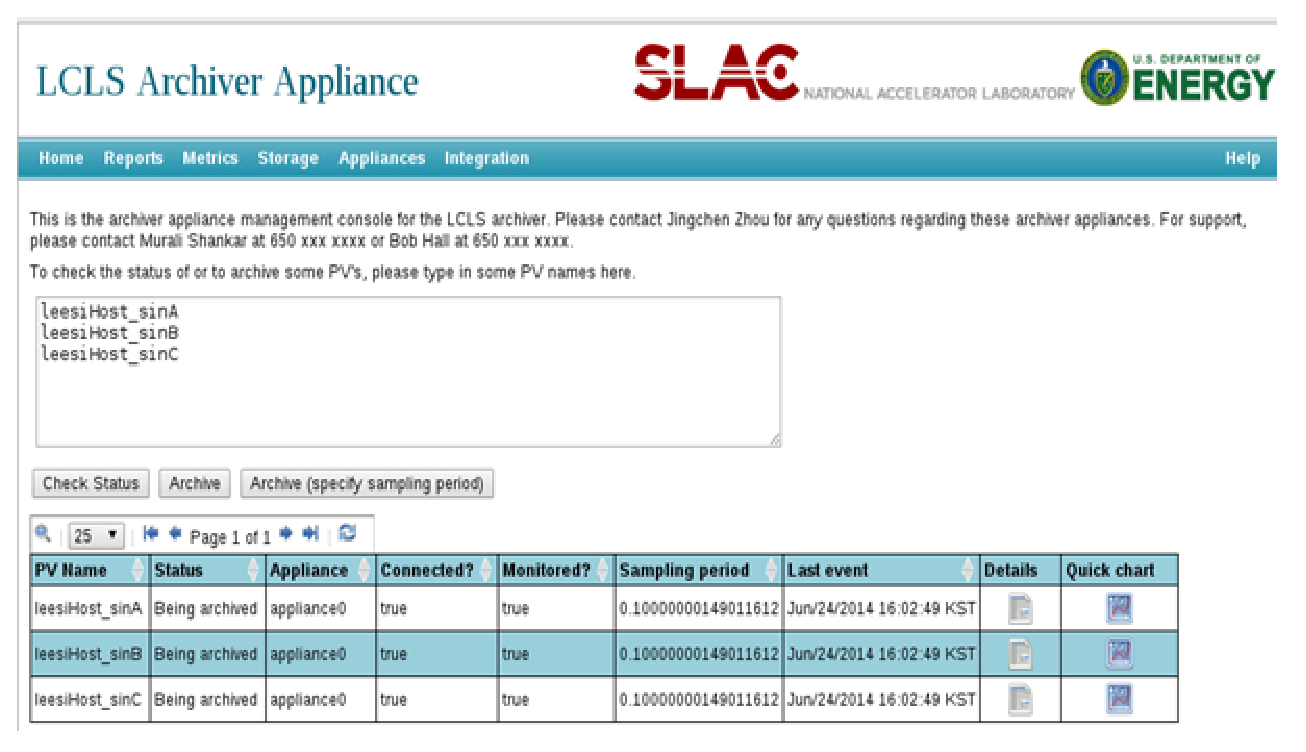
\includegraphics[width=0.85\textwidth, height=0.5\textwidth]{./images/image-5.eps}
		\caption{Management Archiver Appliance}
		\label{fig:mgmt_appliance} 
	\end{figure}
	
\clearpage	

	\item Report 메뉴 \\
	그림 \ref{fig:report}에서 보여지듯이 현재 Appliances에 적용된 PVs에 대한 정보를 여러가지 형식에 따라 list한다. list된 PV의 "Details" 이미지 버튼을 클릭하면 각 PV의 상세정보 및 기본 파라미터를 설정할 수 있으며, 또한 해당 PV를 일시 정지 및 재기동 또는 archive list에서 삭제를 할 수 있다. 상세화면의 각 Attribute에 대한 설명은 본 문서에서는 생략한다.
	\begin{figure}[h!]
		\centering
		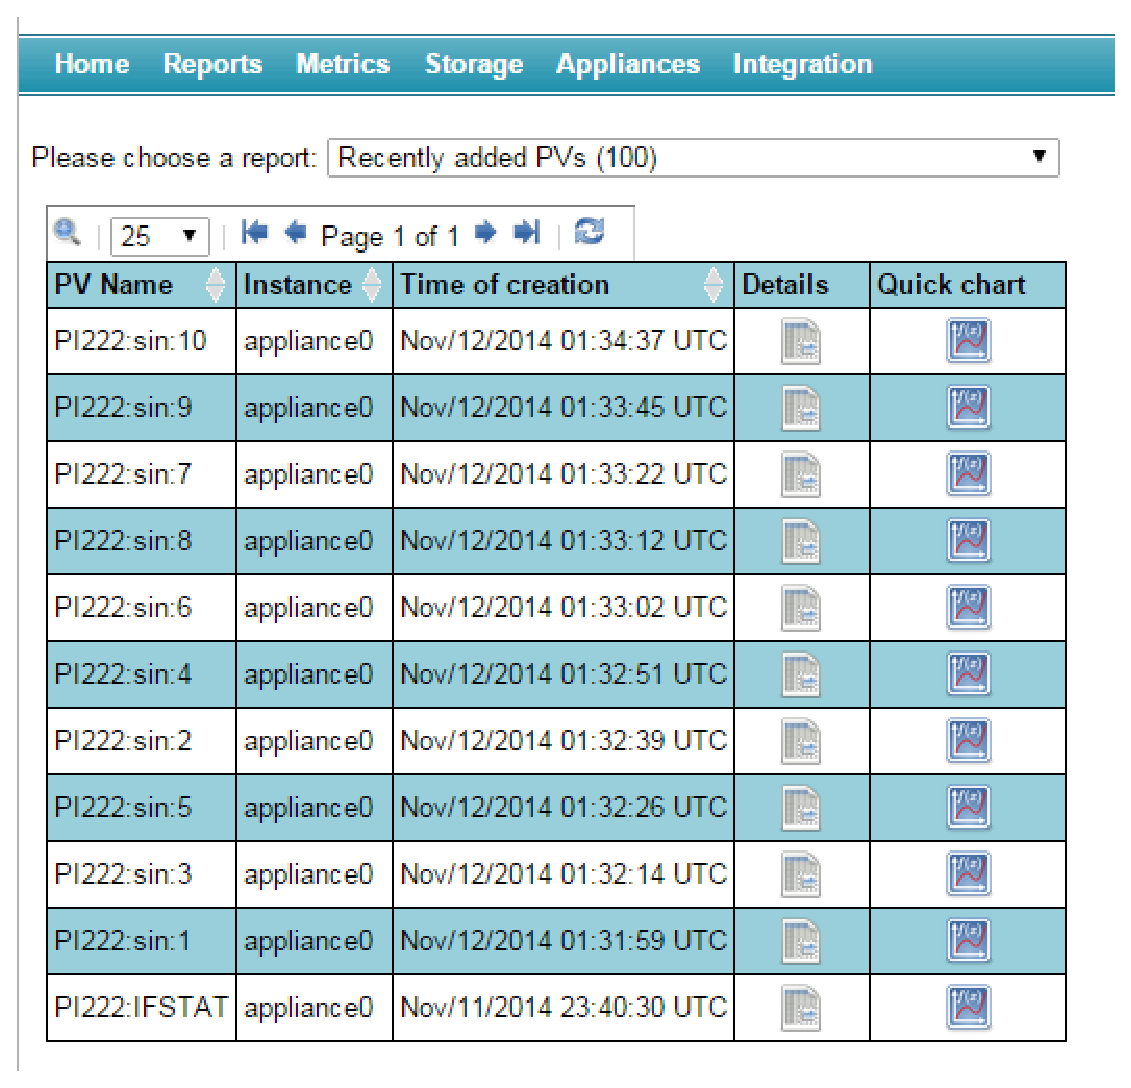
\includegraphics[width=0.85\textwidth, height=0.6\textwidth]{./images/report.eps}
		\caption{Report 메뉴}
		\label{fig:report} 
	\end{figure}
\clearpage

	\item Metrics 메뉴 \\
	그림 \ref{fig:metrics}와 clustered appliances의 각 appliance에 대한 속성을 보여준다. 주요내용(Instance Name, Status, PV Count, Connected Count, Event Rate, Data Rate, Engine write thread, Max ETL)은 화면 상단에 요약되어 보여지며, 하단의 내용은 appliance가 사용하고 있는 스토리지 영역에서 자원사용에 대한 성능 지표를 나타내는 속성 값을 의미한다.

	\begin{figure}[h!]
		\centering
		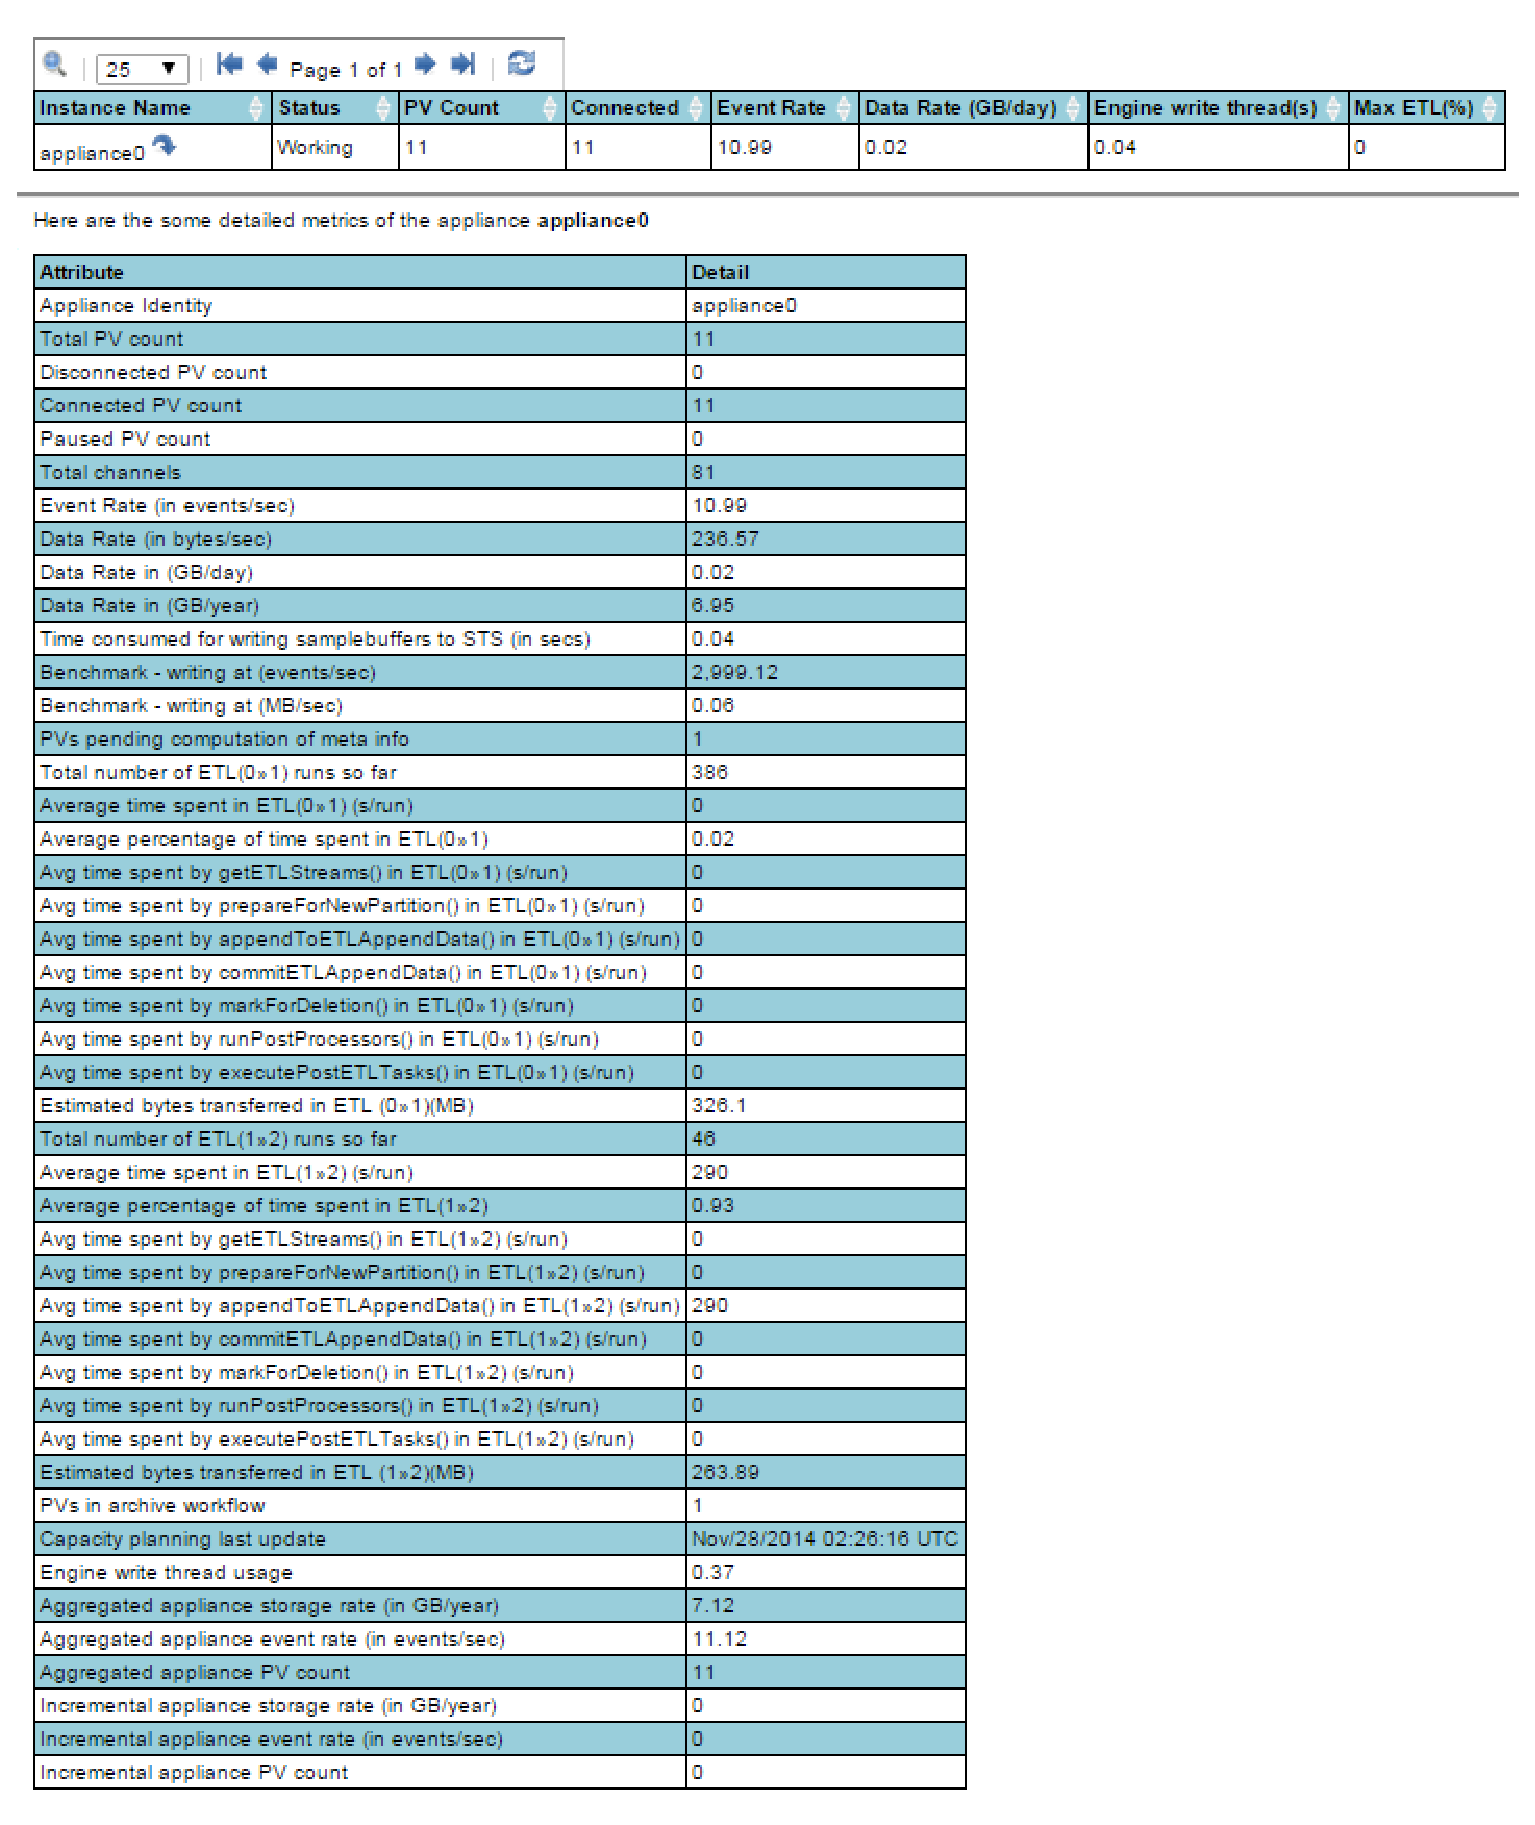
\includegraphics[width=0.85\textwidth, height=0.8\textwidth]{./images/metrics.eps}
		\caption{Metrics 메뉴}
		\label{fig:metrics} 
	\end{figure}
\clearpage

	\item Storage 메뉴 \\
	그림 \ref{fig:storage}는 각 appliance의 스토리지 세 영역(STS, MTS, LTS)에서 사용 되어지고 있는 자원에 대한 주요 내용이다.
	
	\begin{figure}[h!]
		\centering
		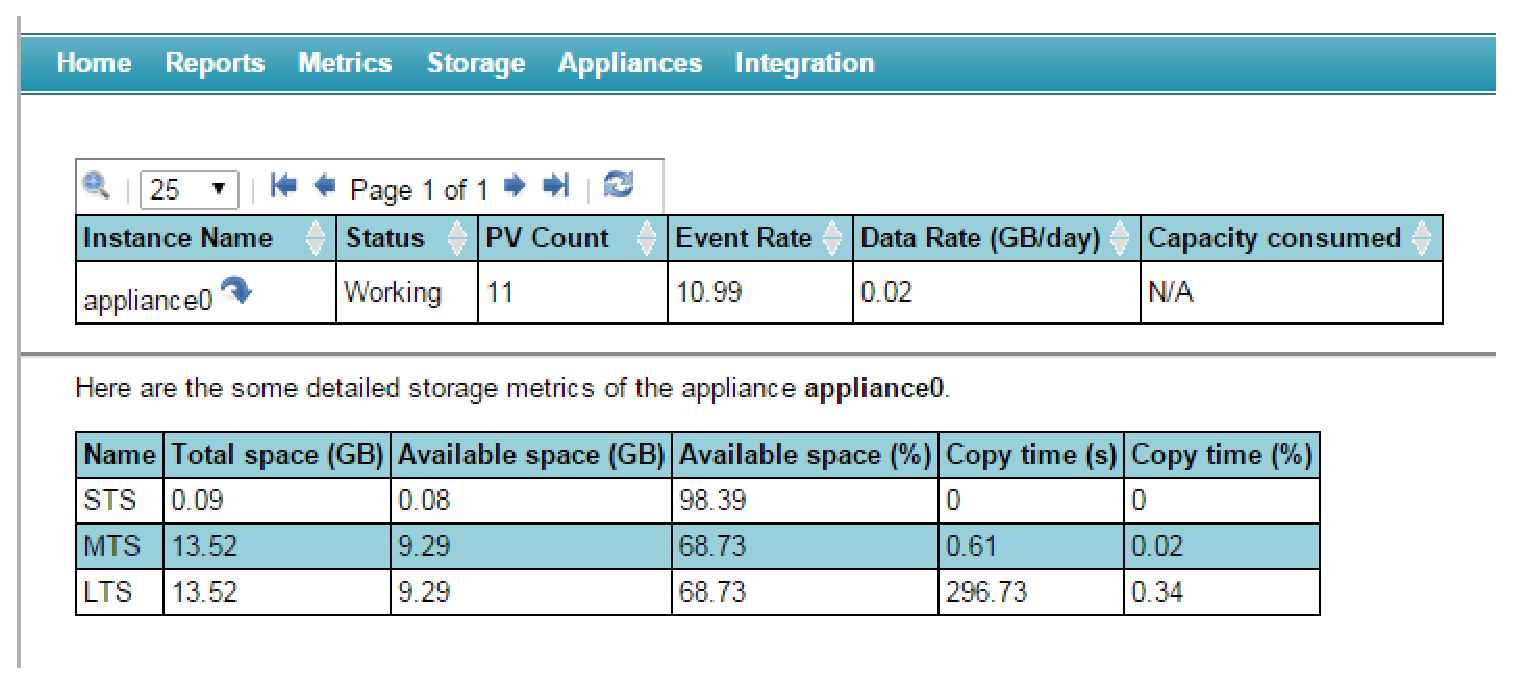
\includegraphics[width=0.85\textwidth, height=0.3\textwidth]{./images/storage.eps}
		\caption{Storage 메뉴}
		\label{fig:storage} 
	\end{figure}

	\item Appliances 메뉴 \\
	그림 \ref{fig:appliance}는 MGMT 모듈을 제외한 주요 세 가지 모듈(Engine, Retrieval, ETL)에 대한 메모리 heap 사용량을 보인다. 
	\begin{figure}[h!]
		\centering
		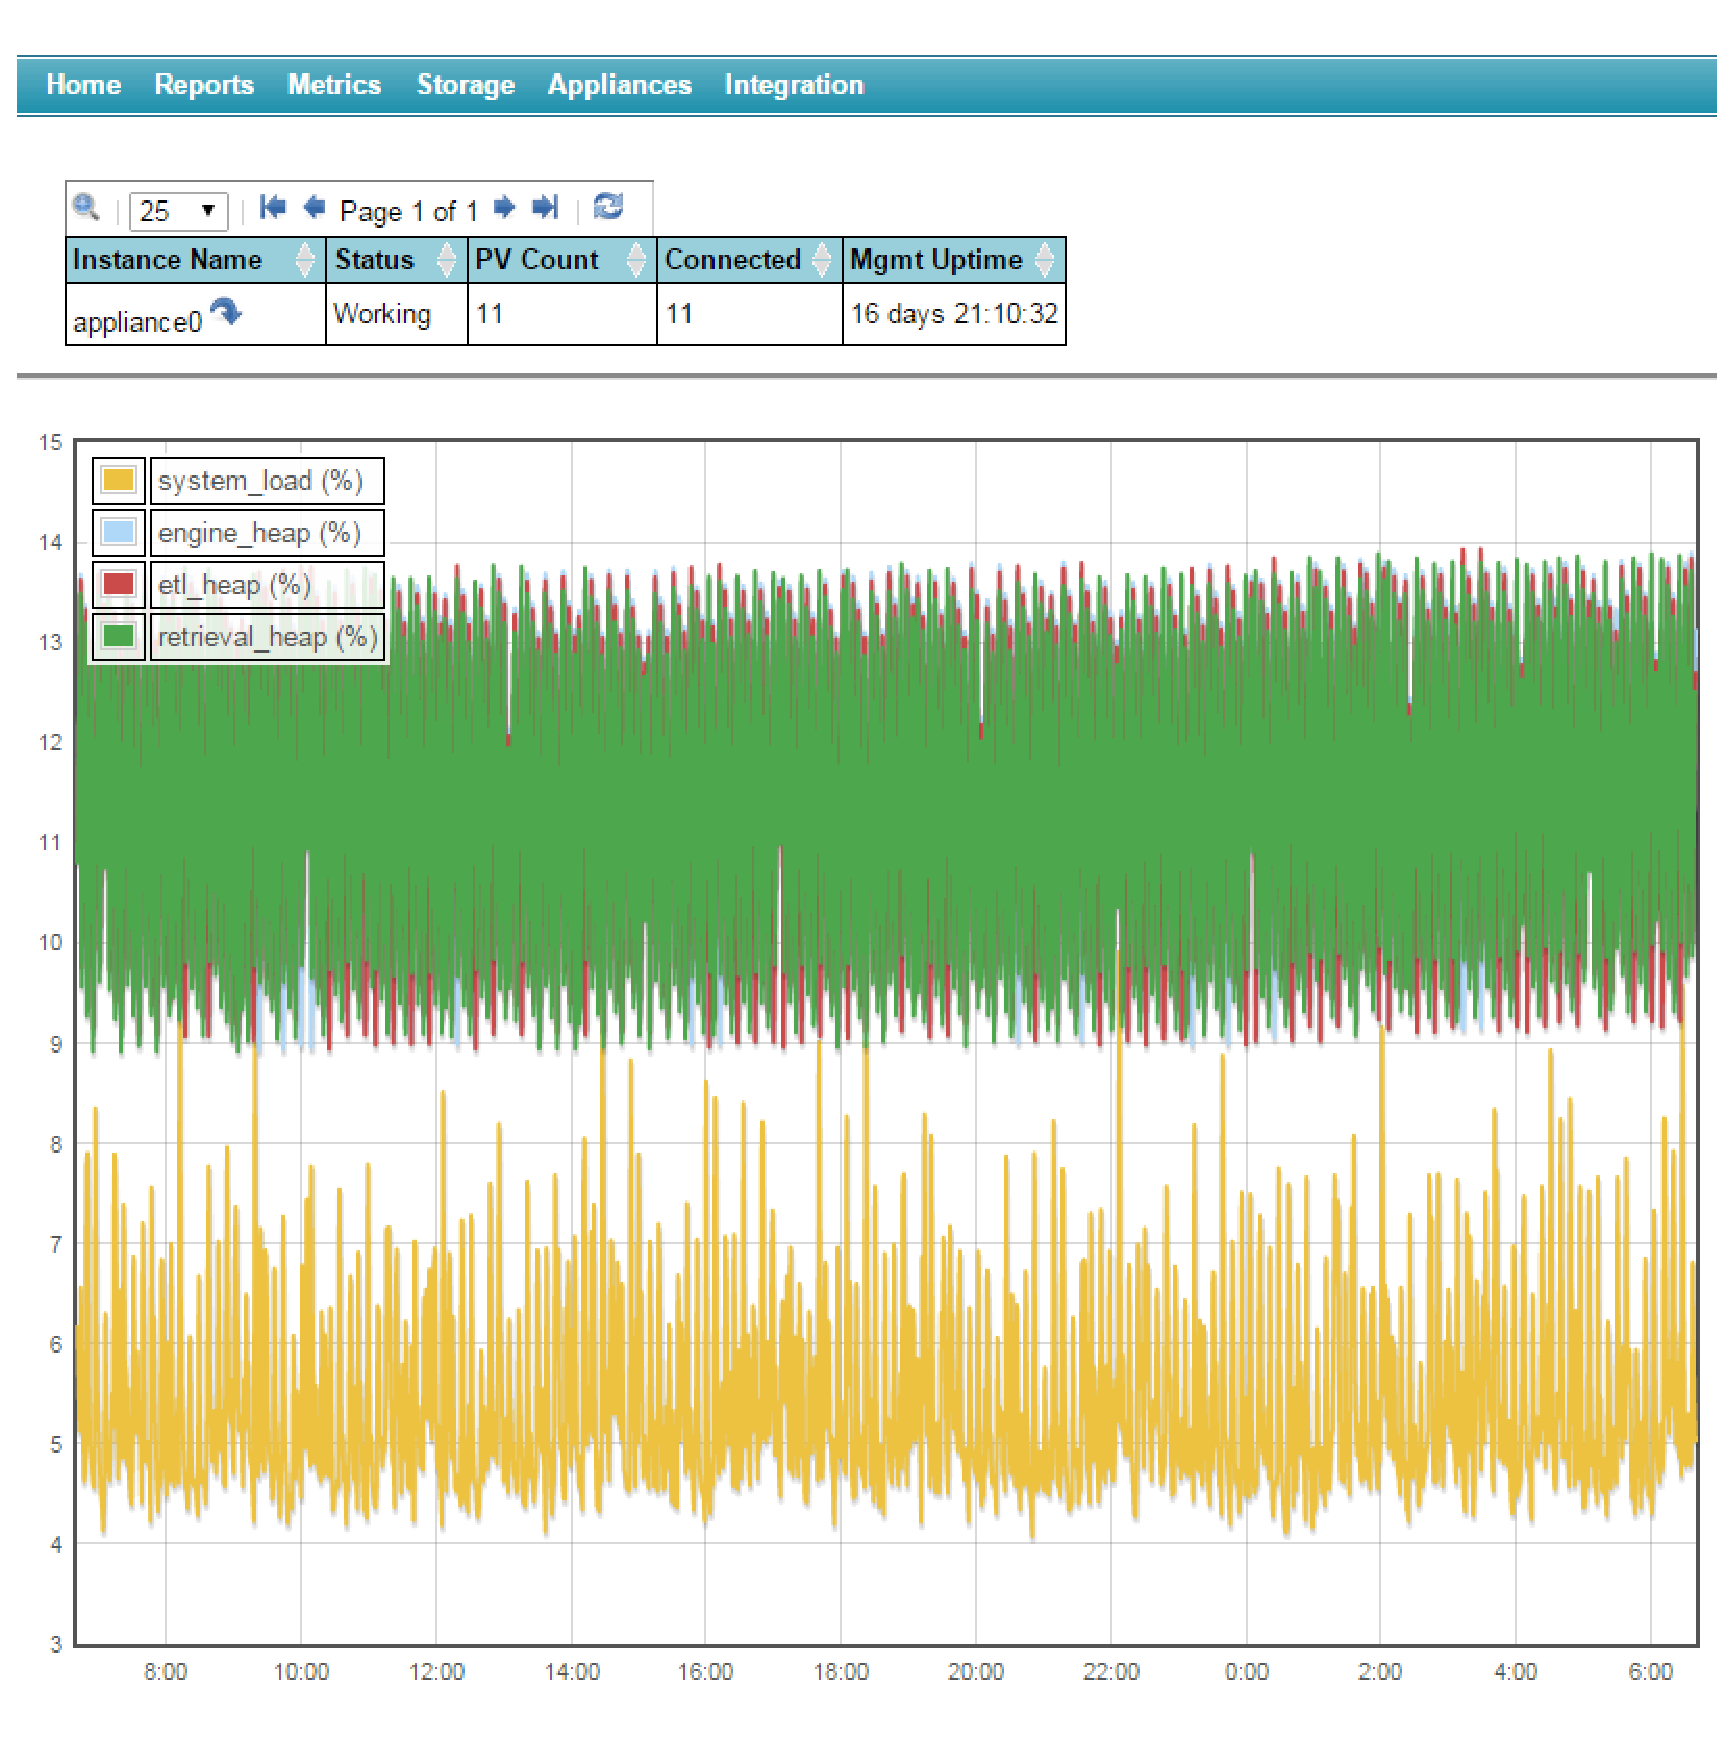
\includegraphics[width=0.85\textwidth, height=0.45\textwidth]{./images/appliance.eps}
		\caption{Appliances 메뉴}
		\label{fig:appliance} 
	\end{figure}
\clearpage
	\item Integration 메뉴 \\
	그림 \ref{fig:integration}는 기존 classic channel archiver의 환경파일을 Load 하거나 데이터를 추출하기 위한 설정메뉴 이다.
	\begin{figure}[h!]
		\centering
		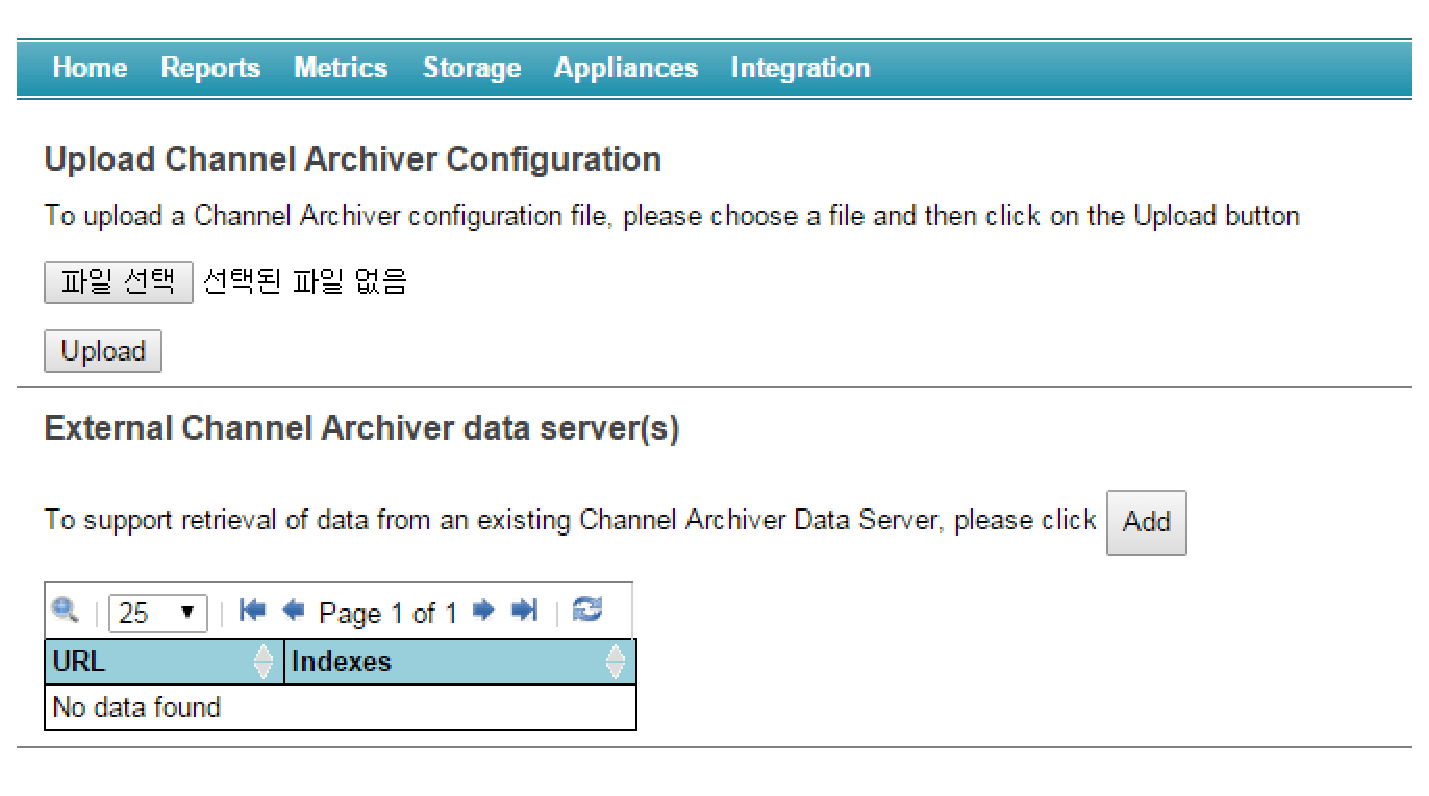
\includegraphics[width=0.85\textwidth, height=0.3\textheight]{./images/integration.eps}
		\caption{Integration 메뉴}
		\label{fig:integration} 
	\end{figure}
\end{itemize}

이렇게 구성된 Single Archiver Appliance는 그림 \ref{fig:multi_appliance}에서 여러 노드로 확장하여 Multiple Archiver Appliances로 구성 가능하다.

\begin{figure}[h!]
	\centering
	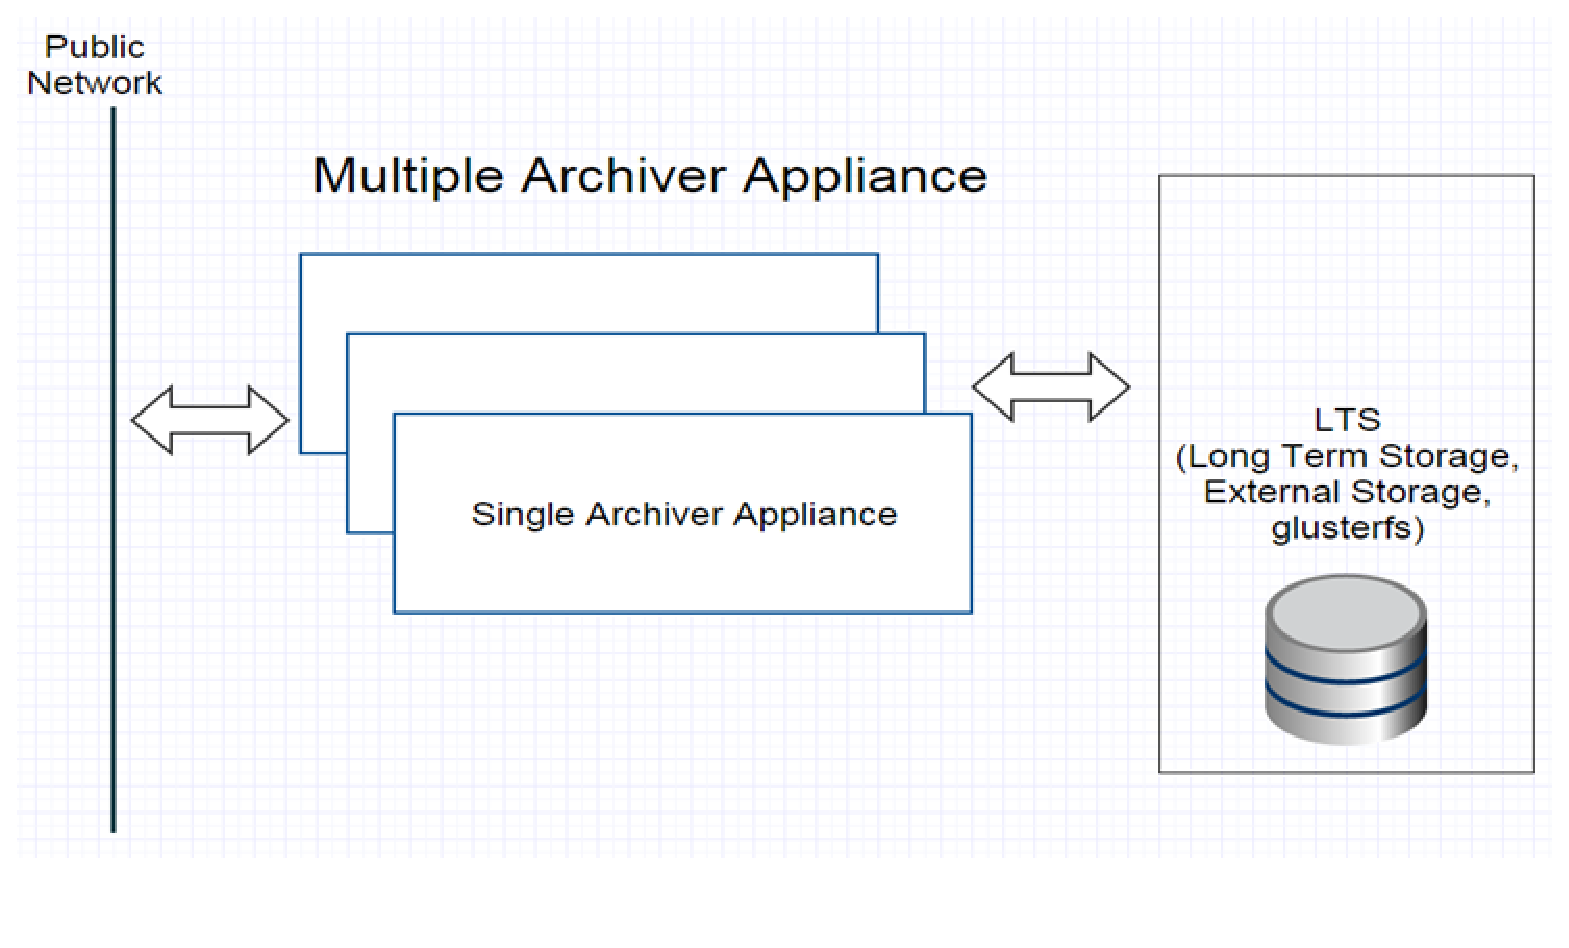
\includegraphics[width=0.85\textwidth, height=0.3\textheight]{./images/image-4.eps}
	\caption{Multiple Archiver Appliance}
	\label{fig:multi_appliance} 
\end{figure}

Multiple Archiver Appliances 구성을 위하여는 appliances 설정 파일을 구성하여야 한다. 설정 파일의 이름은 아래와 같은 환경변수에 저장이 되어야 하며 모든 노드에 동일한 설정 파일과 환경변수가 적용되어야 한다.
\begin{lstlisting}[style=termstyle]
$>export ARCHAPPL_APPLIANCES=/usr/local/archiver_appliance/appliances.xml
\end{lstlisting}


\chapter{Archiver Appliance 설치}
Archiver Appliance 설치를 위하여 항목 3.2 System 요구사항을 참조한다. System 요구사항에 맞는 소프트웨어가 설치 되었다면 아래 사이트에 접속하여 그림 \ref{fig:appli_download}에서 archiveviewer.jar와 최신 버전의 Appliance snapshot 항목을 다운로드 한다.
\begin{lstlisting}[style=termstyle]
http://sourceforge.net/projects/epicsarchiverap/files/snapshots/
\end{lstlisting}
\begin{figure}[h!]
	\centering
	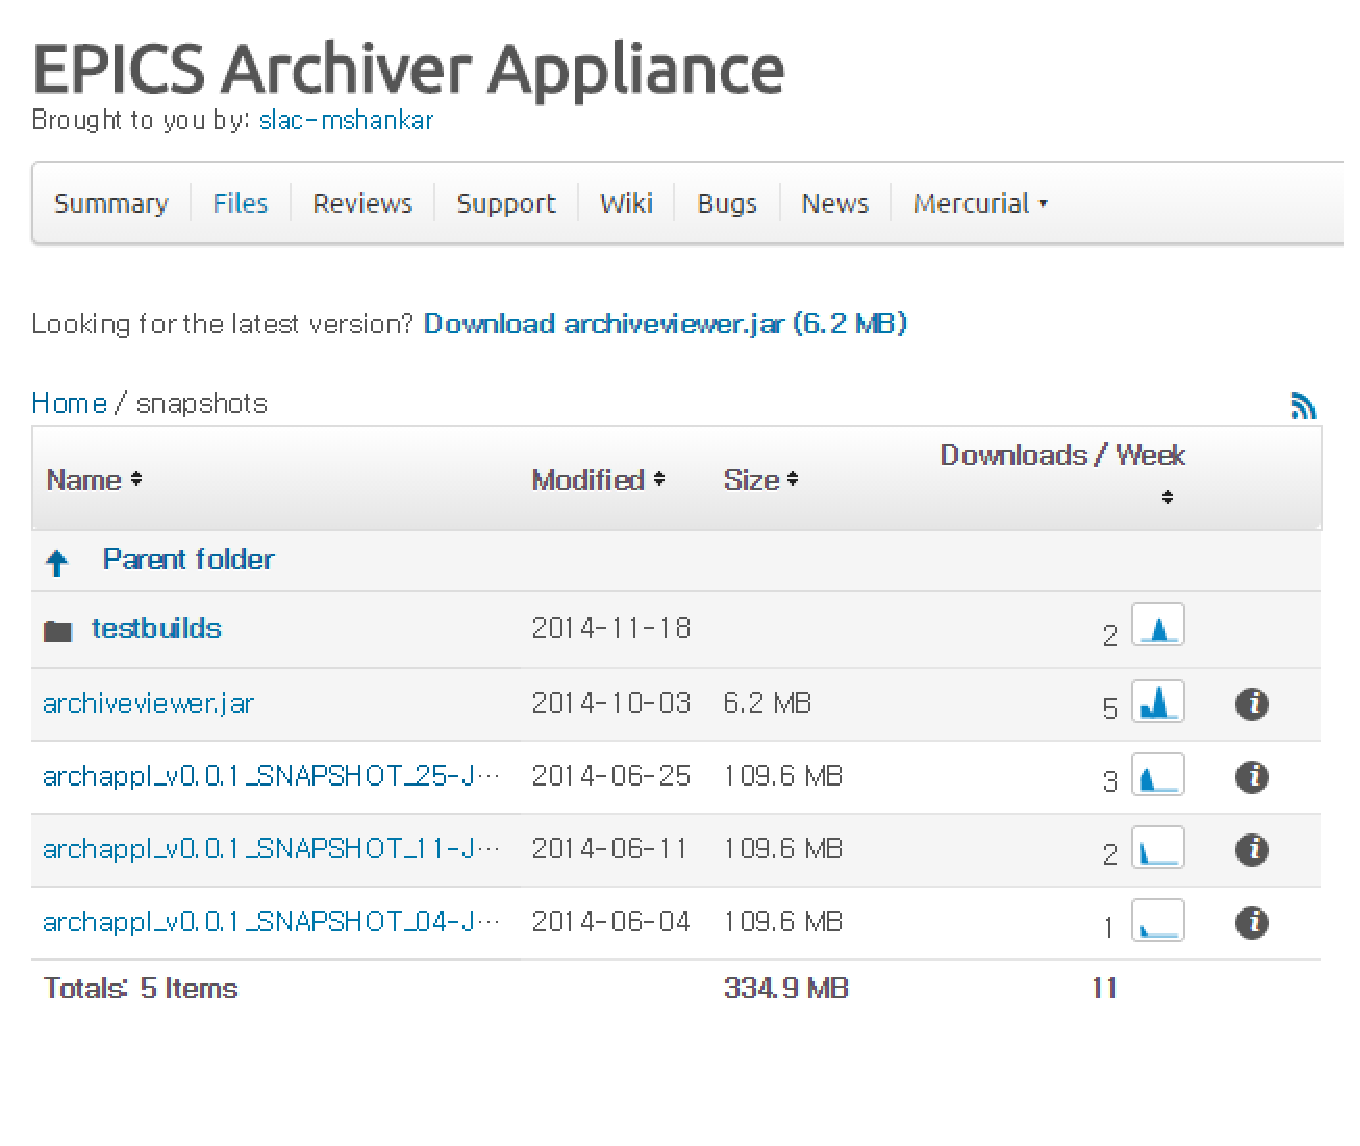
\includegraphics[width=0.65\textwidth, height=0.25\textheight]{./images/appli_download.eps}
	\caption{Archiver Appliance Download}
	\label{fig:appli_download} 
\end{figure}
archiveviwer.jar 파일은 EPICS community site에서 제공되는 것에 google protocol buffer를 사용하여 개발된 모듈이 추가적인 플러그인 모듈로 포함되어 있다.  해당 파일은 소스파일 없이 java compiled class 파일만 제공된다. 다운로드한 파일을 아래와 같이 압축을 풀면 그림 \ref{fig:appli_tree}와 같은 내용을 볼수 있다.

\begin{lstlisting}[style=termstyle]
$>tar xvfz archappl_v0.0.1_SNAPSHOT_11-June-2014T10-57-25.tar.gz
\end{lstlisting}

그림 \ref{fig:appli_tree}에서 보듯이 상위에서 설명한 4개의 모듈(engine, retrieval, etl, mgmg)이 WAR(Web ARchiving) 파일로 java compiled class 파일로 압축되어 제공되어 진다.

\begin{figure}[h!]
	\centering
	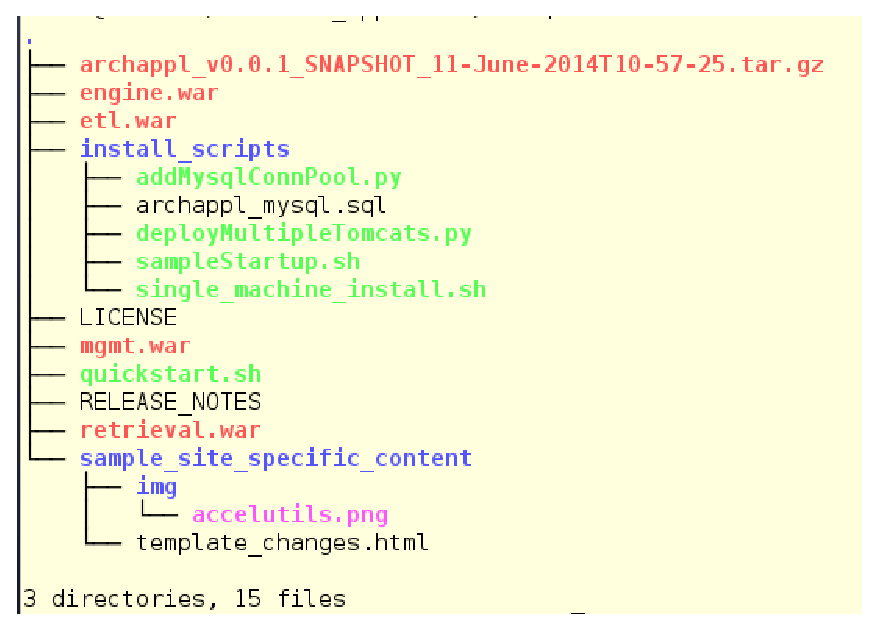
\includegraphics[width=0.75\textwidth, height=0.25\textheight]{./images/appli_tree.eps}
	\caption{Archiver Appliance 설치 Directory}
	\label{fig:appli_tree} 
\end{figure}


\clearpage

해당 모듈의 사용을 위한 License는 아래에 list 한다.

\begin{lstlisting}[style=termstyle]
Copyright (c) 2011 The Board of Trustees of the Leland Stanford Junior University as Operator of the SLAC National Accelerator Laboratory.
Copyright (c) 2011 Brookhaven National Laboratory.
All rights reserved.

EPICS archiver appliance is distributed subject to the following license conditions:
SOFTWARE LICENSE AGREEMENT
Software: EPICS archiver appliance

The "Software", below, refers to EPICS archiver appliance (in either source code, or binary form and accompanying documentation).
Each licensee is addressed as "you" or "Licensee."

The copyright holders shown above and their third-party licensors hereby grant Licensee a royalty-free nonexclusive license,
subject to the limitations stated herein and U.S. Government license rights.

You may modify and make a copy or copies of the Software for use within your organization, if you meet the following conditions:
Copies in source code must include the copyright notice and this Software License Agreement.
Copies in binary form must include the copyright notice and this Software License Agreement in the documentation and/or other materials
provided with the copy.

You may modify a copy or copies of the Software or any portion of it, thus forming a work based on the Software,
and distribute copies of such work outside your organization, if you meet all of the following conditions:
Copies in source code must include the copyright notice and this Software License Agreement;
Copies in binary form must include the copyright notice and this Software License Agreement in the documentation
and/or other materials provided with the copy;
Modified copies and works based on the Software must carry prominent notices stating that you changed specified portions of the Software.

Portions of the Software resulted from work developed under a U.S. Government contract and are subject to the following license:
the Government is granted for itself and others acting on its behalf a paid-up, nonexclusive, irrevocable worldwide license in this computer software to rep

WARRANTY DISCLAIMER. THE SOFTWARE IS SUPPLIED "AS IS" WITHOUT WARRANTY OF ANY KIND.
THE COPYRIGHT HOLDERS, THEIR THIRD PARTY LICENSORS, THE UNITED STATES, THE UNITED STATES DEPARTMENT OF ENERGY,
AND THEIR EMPLOYEES: 
(1) DISCLAIM ANY WARRANTIES, EXPRESS OR IMPLIED, INCLUDING BUT NOT LIMITED TO ANY IMPLIED WARRANTIES OF MERCHANTABILITY,
FITNESS FOR A PARTICULAR PURPOSE, TITLE OR NON-INFRINGEMENT,
(2) DO NOT ASSUME ANY LEGAL LIABILITY OR RESPONSIBILITY FOR THE ACCURACY,
COMPLETENESS, OR USEFULNESS OF THE SOFTWARE,
(3) DO NOT REPRESENT THAT USE OF THE SOFTWARE WOULD NOT INFRINGE PRIVATELY OWNED RIGHTS,
(4) DO NOT WARRANT THAT THE SOFTWARE WILL FUNCTION UNINTERRUPTED, THAT IT IS ERROR-FREE OR THAT ANY ERRORS WILL BE CORRECTED.

LIMITATION OF LIABILITY. IN NO EVENT WILL THE COPYRIGHT HOLDERS, THEIR THIRD PARTY LICENSORS,
THE UNITED STATES, THE UNITED STATES DEPARTMENT OF ENERGY, OR THEIR EMPLOYEES:
BE LIABLE FOR ANY INDIRECT, INCIDENTAL, CONSEQUENTIAL, SPECIAL OR PUNITIVE DAMAGES OF ANY KIND OR NATURE,
INCLUDING BUT NOT LIMITED TO LOSS OF PROFITS OR LOSS OF DATA, FOR ANY REASON WHATSOEVER,
WHETHER SUCH LIABILITY IS ASSERTED ON THE BASIS OF CONTRACT, TORT (INCLUDING NEGLIGENCE OR STRICT LIABILITY),
OR OTHERWISE, EVEN IF ANY OF SAID PARTIES HAS BEEN WARNED OF THE POSSIBILITY OF SUCH LOSS OR DAMAGES.
\end{lstlisting}

\section{Tocat 설치 및 Appliance 환경 구성}
\subsection{Install script를 사용한 설치}
Archiver Appliance 구성은 기본적으로 하나의 노드를 기준으로 설치된다. 상위 항목에서 압축해제된 디렉토리 중 install\_scripts 디렉토리를 보면 아래와 같이 2개의 shell 프로그램, 2개의 python 프로그램과 1개의 sql 파일로 구성되어 있다.

\begin{lstlisting}[style=termstyle]
.
|-- addMysqlConnPool.py
|-- archappl_mysql.sql
|-- deployMultipleTomcats.py
|-- sampleStartup.sh
`-- single_machine_install.sh
\end{lstlisting}
각 파일의 역할을 보면,
\begin{itemize}
	\item single\_machine\_install.sh \\
	single appliance 노드로 설치 및 설정하는 과정을 진행하는 설치 스크립트이다. (Appendix A 참조)
	\item sampleStartup.sh \\
	single 노드 또는 multi 노드로 clustered appliances가 구성된 후 4개의 모듈(engine, retrieval, etl, mgmt)을 노드 별로 구동한다. (Appendix B 참조)
	\item deployMultipleTomcats.py \\
	ARCHAPP\_APPLIANCES 환경변수에 설정된 appliance 노드들에 관련 software package를 deploy 한다. (Appendix C 참조)
	\item addMysqlConnPool.py \\
	각 appliance 노드들에 필요한 정보를 update 하기 위한 mysql connection pool을 구성한다. (Appendix D 참조)
	\item archapp\_mysql.sql \\
	appliance 노드 설정에 필요한 MySQL table을 생성한다. (Appendix E 참조)
\end{itemize}

\subsection{스토리지 영역 구성}
Archiver Appliance에서 사용하는 세 스토리지 영역의 구성 방법은 아래와 같다.
\begin{itemize}
	\item STS \\
	PlainPBStoragePlugin 모듈에서 사용하는 데이터 영역으로 ARCHAPPL\_SHORT\_TERM\\\_FOLDER 쉘 환경 변수에 할당되는 영역에 1 hour의 데이터가 저장된다.
	\begin{lstlisting}[style=termstyle]
	ARCHAPPL_SHORT_TERM_FOLDER=/run/shm/shortterm/
	\end{lstlisting}
	\item MTS \\
	PlainPBStoragePlugin 모듈에서 사용하는 데이터 영역으로 ARCHAPPL\_MEDIUM\_TERM\\\_FOLDER 쉘 환경 변수에 할당되는 영역에 1 day의 데이터가 저장된다.
	\begin{lstlisting}[style=termstyle]
	ARCHAPPL_MEDIUM_TERM_FOLDER=/usr/local/mid-term/
	\end{lstlisting}
	\item LTS \\
	PlainPBStoragePlugin 모듈에서 사용하는 데이터 영역으로 ARCHAPPL\_LONG\_TERM\\\_FOLDER 쉘 환경 변수에 할당되는 영역에 1 year의 데이터가 저장된다.
	\begin{lstlisting}[style=termstyle]
	ARCHAPPL_LONG_TERM_FOLDER=/mnt/glusterfs/long-term/
	\end{lstlisting}
\end{itemize}
세가지 형태의 스토리지 영역을 체계적으로 관리하기 위하여 /archStorage 를 생성 후 아래 구성 예와 같이 symbolic link를 설정한 후 세 영역에 대한 환경 변수를 설정한다.

\begin{lstlisting}[style=termstyle]
$>mkdir ~/archStorage
$>ln -s /dev/shm /archStorage/sts
$>ln -s /ssd /archStorage/mts
$>ln -s /mnt/glusterfs/LTS /archStorage/lts
$>cd ~/archStorage/
$archStorage>ls -lrt
-rwxrwxrwx 1 silee silee 4096 Jun 11 10:58 sts -> /rus/shm
-rwxrwxrwx 1 silee silee 4096 Jun 11 10:58 mts -> /ssd
-rwxrwxrwx 1 silee silee 4096 Jun 11 10:58 lts -> /mnt/glusterfs/LTS
export ARCHAPPL\_SHORT\_TERM\_FOLDER=/archStorage/sts
export ARCHAPPL\_MEDIUM\_TERM\_FOLDER=/archStorage/mts
export ARCHAPPL\_LONG\_TERM\_FOLDER=/archStorage/lts
\end{lstlisting} 


\subsection{Appliance 구성}
아래 appliances 설정 파일을 보면 각 appliance 노드간의 모듈별 통신을 위한 환경을 설정한다. 설정 파일의 각 appliance 섹션은 하나의 appliance 노드에 설정 되어야할 모듈 통신의 내용을 보여준다. cluster inetport는 appliance 정보에 대한 통신을 위한 구성이며, mgmt, engine, etl 및 retrieval 항목은 아파치 톰캣 framework간의 http 프로토콜을 사용하여 각 appliance 노드의 모듈간 통신을 위한 설정이다. 각 appliance의 노드는 전체 클러스터에서 필요시 추가적으로 확장할 수 있는 확장성을 가지며 운영 중 하나의 노드가 fail이 발생 하더라도 다른 노드의 서비스에는 영향을 주지 않는다. 주의 할 점은 각 appliance 노드 이름은 클러스터 내에서 고유하여야 하면 cluster\_inetport는 모든 노드에서 동일하여야 한다. 이 통신 포트는 각 노드들 간의 통신이 이루어진다. mgmt\_url, engine\_url, retrieval\_url 및 data\_retrieval\_url의 통신 포트는 모든 노드에서 동일하여야 하는 상황은 아니지만 가능한 동일하게 사용하는 것이 좋다. 부득히 다른 포트를 사용해야 하는 노드가 발생 한다면 mgmt\_url port를 최소 번호로 1씩 증가하는 port를 사용한다는 내부 규약에 맞추어 사용하는 것이 appliance 운영에 혼선을 막을 수 있다. 또한, 데이터 추출을 위하여 두개의 retrieval\_url이 사용 되는데, retrieval\_url은 mgmt 모듈과 retrieval 모듈 간 통신을 위한 설정이며, data\_retrieval\_url은 retrieval data client 모듈과 cluster 노드 간의 통신을 위한 설정이다. 각 노드는 apache의 mod-proxy-balancer는 cluster의 모든 appliances 노드들 간의 load-balanace에 사용된다. 현 "apache + tocat"의 mod-proxy-balancer는 AJP라 불리는 binary protocol을 사용하는데 이는 AJP protocol 전체를 지원하는 모듈은 아니므로, 추가적인 site 특성에 맞는 추가적인 load balancer를 구현하려 한다면 주의해야 한다.

\begin{lstlisting}[style=termstyle]
<appliances>
<appliance>
<identity>appliance0</identity>
<cluster_inetport>appliance0_ip_address:16670</cluster_inetport>
<mgmt_url>http://appliance0_ip_address:17665/mgmt/bpl</mgmt_url>
<engine_url>http://appliance0_ip_address:17666/engine/bpl</engine_url>
<etl_url>http://appliance0_ip_address:17667/etl/bpl</etl_url>
<retrieval_url>http://appliance0_ip_address:17668/retrieval/bpl</retrieval_url>
<data_retrieval_url>http://appliance0_ip_address:17668/retrieval</data_retrieval_url>
</appliance>
<appliance>
<identity>appliance1</identity>
<cluster_inetport>appliance1_ip_address:16670</cluster_inetport>
<mgmt_url>http://appliance1_ip_address:17665/mgmt/bpl</mgmt_url>
<engine_url>http://appliance1_ip_address:17666/engine/bpl</engine_url>
<etl_url>http://appliance1_ip_address:17667/etl/bpl</etl_url>
<retrieval_url>http://appliance1_ip_address:17668/retrieval/bpl</retrieval_url>
<data_retrieval_url>http://appliance1_ip_address:17668/retrieval</data_retrieval_url>
</appliance>
<appliance>
<identity>appliance2</identity>
<cluster_inetport>appliance2_ip_address:16670</cluster_inetport>
<mgmt_url>http://appliance2_ip_address:17665/mgmt/bpl</mgmt_url>
<engine_url>http://appliance2_ip_address:17666/engine/bpl</engine_url>
<etl_url>http://appliance2_ip_address:17667/etl/bpl</etl_url>
<retrieval_url>http://appliance2_ip_address:17668/retrieval/bpl</retrieval_url>
<data_retrieval_url>http://appliance2_ip_address:17668/retrieval</data_retrieval_url>
</appliance>
</appliances>
\end{lstlisting}

\section{Apache 데몬 설정}
상위 System 요구사항에 명시된 버전의 Apache Tomcat을 설치 하였다면, TOMCAT\_HOME 환경 변수를 Site 상황에 맞게 설정한다. 설치된 Tomcat의 Home 디렉토리에서 conf/server.xml 설정 파일 중에서 아래에 해당 하는 HTTP 설정 중 port 번호(디폴트 8080)를 mgmt 모듈에서 설정한 port 번호(17665)로 변경한다. 8080 포트는 일반적으로 알려진 포트이므로 appliance를 위한 포트 설정으로 변경하기 위함이다.
\begin{lstlisting}[style=termstyle]
    <Connector port="17665" protocol="HTTP/1.1" connectionTimeout="20000"
    redirectPort="8443" />
\end{lstlisting}

또한 아래와 같이 AJP Connector에 대한 port 설정 부분은 주석처리 또는 해당 라인을 제거한다.
\begin{lstlisting}[style=termstyle]
<!-- Define an AJP 1.3 Connector on port 8009 -->
<!-- <Connector port="8009" protocol="AJP/1.3" redirectPort="8443" /> -->
\end{lstlisting}

설정 파일 중 주석처리 또는 제거되지 말아야 할 설정은 Tomcat 서버의 shutdown 명령을 실행 하여야 할 설정이며,
아래와 같다.
\begin{lstlisting}[style=termstyle]
<Server port="8005" shutdown="SHUTDOWN">
\end{lstlisting}

apache 데몬의 log 설정을 위하여 아래와 같이 TOMCAT\_HOME/lib/log4j.properties 파일을 생성하여 편집한다. 
\begin{lstlisting}[style=termstyle]
# Set root logger level and its only appender to A1.
log4j.rootLogger=ERROR, A1
log4j.logger.config.org.epics.archiverappliance=INFO
log4j.logger.org.apache.http=ERROR

# A1 is set to be a DailyRollingFileAppender
log4j.appender.A1=org.apache.log4j.DailyRollingFileAppender
log4j.appender.A1.File=arch.log
log4j.appender.A1.DatePattern='.'yyyy-MM-dd

# A1 uses PatternLayout.
log4j.appender.A1.layout=org.apache.log4j.PatternLayout
log4j.appender.A1.layout.ConversionPattern=%-4r [%t] %-5p %c %x - %m%n
\end{lstlisting}

apache 서비스에 대한 monitoring 및 management를 위하여 bin/commons-daemon-native.tar.gz 파일의 압축 해제 후 컴파일 하여 jsvc 실행 파일을 TOMCAT\_HOME/bin에 복사한다.

\begin{lstlisting}[style=termstyle]
$>tomcat7/apache-tomcat-7.0.54/bin# tar xvfz commons-daemon-native.tar.gz 
$>tomcat7/apache-tomcat-7.0.54/bin# cd commons-daemon-1.0.15-native-src/
$>tomcat7/apache-tomcat-7.0.54/bin/commons-daemon-1.0.15-native-src# cd unix/
$>tomcat7/apache-tomcat-7.0.54/bin/commons-daemon-1.0.15-native-src/unix# cp jsvc $TOMCAT_HOME/bin
\end{lstlisting}

\section{MySQL 설치 및 설정}
각 appliance 노드에서 추가 및 변경된 설정 내용에 대하여 MySQL database에 table로 저장된다. 이러한 구성을 위하여 각 노드에 MySQL database를 아래와 같이 설치하고 노드에서 사용될 database를 생성한다.
\begin{lstlisting}[style=termstyle]
#>aptitude install mysql-server 
\end{lstlisting}

\begin{lstlisting}[style=termstyle]
$>mysql -u user-name -p
passwd:
mysql>create database archappl;
mysql>grant all on archappl.* to 'archappl'@localhost indentified by 'password';
\end{lstlisting}
archappl database를 생성후 mgmt 모듈 안의 install/archappl\_mysql.sql를 실행하면 새로운 schema가 아래와 같이 생성된다.

\begin{lstlisting}[style=termstyle]
mysql> use archappl;
Reading table information for completion of table and column names
You can turn off this feature to get a quicker startup with -A
Database changed

mysql> show tables;
+---------------------+
| Tables_in_archappl  |
+---------------------+
| ArchivePVRequests   |
| ExternalDataServers |
| PVAliases           |
| PVTypeInfo          |
+---------------------+
4 rows in set (0.00 sec)
\end{lstlisting}
각 Table은 아래와 같은 목적에 따라 설정을 저장한다.
\begin{itemize}
	\item PVTypeInfo \\
	PV의 archiving parameter에 대한 정보를 저장
	\item PVAliases \\
	EPICS PV의 alias mapping 정보를 저장
	\item ExternalDataServers \\
	External data server에 대한 정보를 저장
	\item ArchivePVRequests \\
	Pending 상태에 있는 PV에 대한 archive 요청
\end{itemize}

각 appliance 노드들간에 상위의 table에 대한 정보를 저장하기 위하여 JDBC connector(mysql-connector-java-x.x.xx.tar.gz)를 사용한다. 해당 모듈은 
아래 사이트에서 다운로드하여 TOMCAT\_HOME/lib에 설치한다. 

\begin{lstlisting}[style=termstyle]
http://dev.mysql.com/downloads/connector/j/
\end{lstlisting}

JDBC 설치 후 TOMCAT\_HOME/conf/context.xml에 jdbc/archappl라는 이름을 갖는 connection pool을 구성하며,구성 방법은 아래와 같다. 아래에서 "Resource name" 속성을 제외하고 각 속성은 Site에 최적화된 옵션으로 수정 될 수 있다.

\begin{lstlisting}[style=termstyle]
<Context>

<!-- Default set of monitored resources -->
<WatchedResource>WEB-INF/web.xml</WatchedResource>
	<Resource   name="jdbc/archappl"
		auth="Container"
		type="javax.sql.DataSource"
		factory="org.apache.tomcat.jdbc.pool.DataSourceFactory"
		username="archappl"
		password="XXXXXXX" 
		testWhileIdle="true"
		testOnBorrow="true"
		testOnReturn="false"
		validationQuery="SELECT 1"
		validationInterval="30000"
		timeBetweenEvictionRunsMillis="30000"
		maxActive="10" 
		minIdle="2" 
		maxWait="10000" 
		initialSize="2"
		removeAbandonedTimeout="60"
		removeAbandoned="true"
		logAbandoned="true"
		minEvictableIdleTimeMillis="30000" 
		jmxEnabled="true"
		driverClassName="com.mysql.jdbc.Driver"
		url="jdbc:mysql://localhost:3306/archappl"
	/>
</Context>
\end{lstlisting}

\section{Appliance 노드 설정 및 실행}
\subsection {4개의 web 모듈을 위한 Tomcat container 설정}
 mgmt 모듈의 install/deployMultipleTomcats.py 파일은 정의된 appliances.xml 파일에 따라 tomcat containers를 생성한다. 이 script를 실행하기 위해서는 아래 환경변수가 설정되어 있음을 확인한다.
 \begin{itemize}
 	\item TOMCAT\_HOME \\
 	Tomcat java 설치 Home 디렉토리
 	\item ARCHAPP\_APPLIANCES \\
 	appliances.xml 파일 설치 경로 
 	\item ARCHAPPL\_MYIDENTITY \\
 	appliance\_0 ~ appliance\_n 까지의 appliance 노드의 고유 이름
 \end{itemize}
 
 이 스크립트의 실행 예는 아래와 같다.
 
\begin{lstlisting}[style=termstyle]
$>export TOMCAT_HOME=$HOME/tomcat
$>export ARCHAPPL_APPLIANCES=$HOME/appliance/appliance.xml
$>export ARCHAPPL_MYIDENTITY=appliance_0
$mgmt/install>chmod +x deployMultipleTomcats.py
$mgmt/install>./deployMultipleTomcats.py $HOME/appliance/continers
Using
    tomcat installation at /home/silee/tomcat
    to generate deployment for appliance appliance_0
    using configuration info from /home/silee/appliance/appliances.xml
    into folder /home/silee/appliance/containers
The stop/start ports for the new instanace will being at 16001
Generating tomcat folder for mgmt in location /home/silee/appliance/containers/mgmt
Generating tomcat folder for engine in location /home/silee/appliance/containers/engine
Generating tomcat folder for etl in location /home/silee/appliance/containers/etl
Generating tomcat folder for retrieval in location /home/silee/appliance/containers/retrieval

$>ls -lrt /home/silee/containers
drwxr-xr-x 1 silee silee 4096 Jun 11 13:41 mgmt/
drwxr-xr-x 1 silee silee 4096 Jun 11 13:41 engine/
drwxr-xr-x 1 silee silee 4096 Jun 11 13:41 etl/
drwxr-xr-x 1 silee silee 4096 Jun 11 13:41 retrieval/
\end{lstlisting}

위의 설정이 완료 되었다면 single appliance 노드 설치 및 설정이 완료된 상황을 말하며, 노드의 확장은 single 노드 설정의 반복 구성을 완료하면 이루어진다.

\subsection {WAR 파일 배포}
appliance 노드의 4가지의 모듈에 수정 사항이 발생할 경우 아래와 같은 절차로 수정된 모듈을 update 한다. 정의된 4개의 모듈의 container에는 webapps 폴더가 존재한다. 해당 폴더의 war file을 삭제한 후 새롭게 빌드된 war file(예, images, policies, appliances)을 복사한다.
 \begin{itemize}
 	\item 4개의 tomcat container 정지
 	\item 각 container의 webapps/ 밑에서 war 파일 삭제
 	\item 새로 build된 war 파일을 해당 container의 webapps/ 에 복사
 	\item 4개의 tomcat container 기동
 \end{itemize}

\begin{lstlisting}[style=termstyle]
pushd ${DEPLOY_DIR}/mgmt/webapps && rm -rf mgmt*; cp ${WARSRC_DIR}/mgmt.war .; popd; 
pushd ${DEPLOY_DIR}/engine/webapps && rm -rf engine*; cp ${WARSRC_DIR}/engine.war .; popd; 
pushd ${DEPLOY_DIR}/etl/webapps && rm -rf etl*; cp ${WARSRC_DIR}/etl.war .; popd; 
pushd ${DEPLOY_DIR}/retrieval/webapps&&rm -rf retrieval*; cp ${WARSRC_DIR}/retrieval.war .; popd;
\end{lstlisting}

\subsection {Appliance 정지 및 기동}
상위에서 설명한 apache common daemon을 설치하면 jsvc를 사용할 수 있으며 아래와 같은 두 가지의 쉘 펑션을 사용하여 각 container에 대한 기동 및 정지를 실행 할 수 있다. 

\begin{lstlisting}[style=termstyle]
function startTomcatAtLocation() { 
if [ -z "$1" ]; then echo "startTomcatAtLocation called without any arguments"; exit 1; fi
export CATALINA_HOME=${TOMCAT_HOME}
export CATALINA_BASE=$1
echo "Starting tomcat at location ${CATALINA_BASE}"
pushd ${CATALINA_BASE}/logs
${CATALINA_HOME}/bin/jsvc \
-server \
-cp ${CATALINA_HOME}/bin/bootstrap.jar:${CATALINA_HOME}/bin/tomcat-juli.jar \
${JAVA_OPTS} \
-Dcatalina.base=${CATALINA_BASE} \
-Dcatalina.home=${CATALINA_HOME} \
-outfile ${CATALINA_BASE}/logs/catalina.out \
-errfile ${CATALINA_BASE}/logs/catalina.err \
-pidfile ${CATALINA_BASE}/pid \
org.apache.catalina.startup.Bootstrap start
popd
}

function stopTomcatAtLocation() { 
if [ -z "$1" ]; then echo "stopTomcatAtLocation called without any arguments"; exit 1; fi
export CATALINA_HOME=${TOMCAT_HOME}
export CATALINA_BASE=$1
echo "Stopping tomcat at location ${CATALINA_BASE}"
pushd ${CATALINA_BASE}/logs
${CATALINA_HOME}/bin/jsvc \
-server \
-cp ${CATALINA_HOME}/bin/bootstrap.jar:${CATALINA_HOME}/bin/tomcat-juli.jar \
${JAVA_OPTS} \
-Dcatalina.base=${CATALINA_BASE} \
-Dcatalina.home=${CATALINA_HOME} \
-outfile ${CATALINA_BASE}/logs/catalina.out \
-errfile ${CATALINA_BASE}/logs/catalina.err \
-pidfile ${CATALINA_BASE}/pid \
-stop \
org.apache.catalina.startup.Bootstrap 
popd
}

\end{lstlisting}

상위의 쉘 펑션을 통하여 각 container에 대한 기동 및 정지는 아래 예와 같다.

\begin{lstlisting}[style=termstyle]
startTomcatAtLocation ${DEPLOY_DIR}/mgmt
startTomcatAtLocation ${DEPLOY_DIR}/engine
startTomcatAtLocation ${DEPLOY_DIR}/etl
startTomcatAtLocation ${DEPLOY_DIR}/retrieval

stopTomcatAtLocation ${DEPLOY_DIR}/engine
stopTomcatAtLocation ${DEPLOY_DIR}/retrieval
stopTomcatAtLocation ${DEPLOY_DIR}/etl
stopTomcatAtLocation ${DEPLOY_DIR}/mgmt
\end{lstlisting}

상위에서 사용되는 환경 변수 이외에 추가 설정을 보면 아래와 같다.
아래 예에서 JAVA\_OPTS 환경변수는 Java Virtual Machine에 대한 옵션을 설정한다. \\ 또한, LD\_LIBRARY\_PATH 에 대한 설정이 필요한 이유는 appliance 노드가 JCA (Java Channel Access)를 이용하는 경우에 JCA은 C 언어와의 binding 사용하여 구현 되었기 때문에 순수 Java 코드가 아니므로 LD\_LIBRARY\_PATH에 EPICS의 base library 경로와 JCA library 경로를 추가해야 한다. 

\begin{lstlisting}[style=termstyle]
export JAVA_OPTS="-XX:MaxPermSize=128M -XX:+UseG1GC -Xmx4G -Xms4G -ea"
export LD_LIBRARY_PATH=$EPICS_BASE/lib/linux-x86_64:JCA_LIB_PATH
\end{lstlisting}

Archiver appliance에서 사용하는 EPICS channel access는 순수 Java code로 구현된 CAJ 버전과 EPICS base library를 binding하여 사용하는 JCA 두 버전이 있다. engine 모듈의 WEB-INF/classes/archappl.properties 설정 파일에는 아래와 같은 옵션을 설정하여 두 버전 중 하나를 선택한다. CAJ 버전을 사용시 "true" 설정.
\begin{lstlisting}[style=termstyle]
# Use this property to control whether you want to use CAJ or the JNI implementation in JCA.
org.epics.archiverappliance.engine.epics.JCAConfigGen.useCAJ=true
\end{lstlisting}
CAJ 버전을 사용한다면 engine 모듈이 생성하는 log에 아래와 같은 설정을 확인 할 수 있다. 아래의 설정은 EPICS 환경 변수를 appliance engine 모듈이 상속하여 생성하는 것으로 생각된다.

\begin{lstlisting}[style=termstyle]
[JCA Command Thread] INFO config.org.epics.archiverappliance.engine.JCAConfigGen - JCA Configuration
<context class="com.cosylab.epics.caj.CAJContext">
<preemptive_callback>true</preemptive_callback>
<addr_list>10.1.4.173</addr_list>
<auto_addr_list>false</auto_addr_list>
<connection_timeout>30.0</connection_timeout>
<beacon_period>15.0</beacon_period>
<repeater_port>5067</repeater_port>
<server_port>5066</server_port>
<max_array_bytes>80000000</max_array_bytes>
<event_dispatcher class="gov.aps.jca.event.QueueEventDispatcher"/>
</context>
\end{lstlisting}

\clearpage

\chapter{Appliance single 노드 file I/O 성능 시험}
최적의 Archiver Appliance 구축을 위하여는 크게 두가지 관점에서 접근 할 수 있다. 하나는 각 single 노드에서 사용하는 file system의 성능을 극대화 하기 위한 방법이며, 다른 하나는 multiple appliance 노드를 site 전체 관점에서 최적의 환경으로 구성하는 방법이며 이는 Long Term Storage 시스템 설계와 연관된다. Multiple appliance 설치 및 성능 시험은 다음 단계에서 진행 될 예정이며 본 문서에 언급은 생략하기로 한다. 본 문서에는 appliance 성능 시험의 첫 단계로 single appliance 노드를 구축하여 file system 성능 시험을 진행하였다.  

\section{I/O Bandwidth 측정 (dd benchmark)}
Test appliance 노드의 스토리지 영역은 아래와 같이 세가지 영역으로 구성된다.

\begin{itemize}
	\item STS (Short Term Storage) 영역\\
	appliance 노드가 1시간의 분량의 데이터를 저장하기 위하여 memory mapped RAM file system 영역
	\item MTS (Medium Term Storage) 영역 \\
	appliance 노드가 1일 분량의 데이터를 저장하기 위한 disk 영역 ext4 file system (SATA disk)
	\item LTS (Long Term Storage) 영역 \\
	appliance 노드가 1일 이상의 데이터를 저장하기 위한 외부 저장 영역 gluster file system (Network)
\end{itemize}

\begin{figure}[h!]
	\centering
	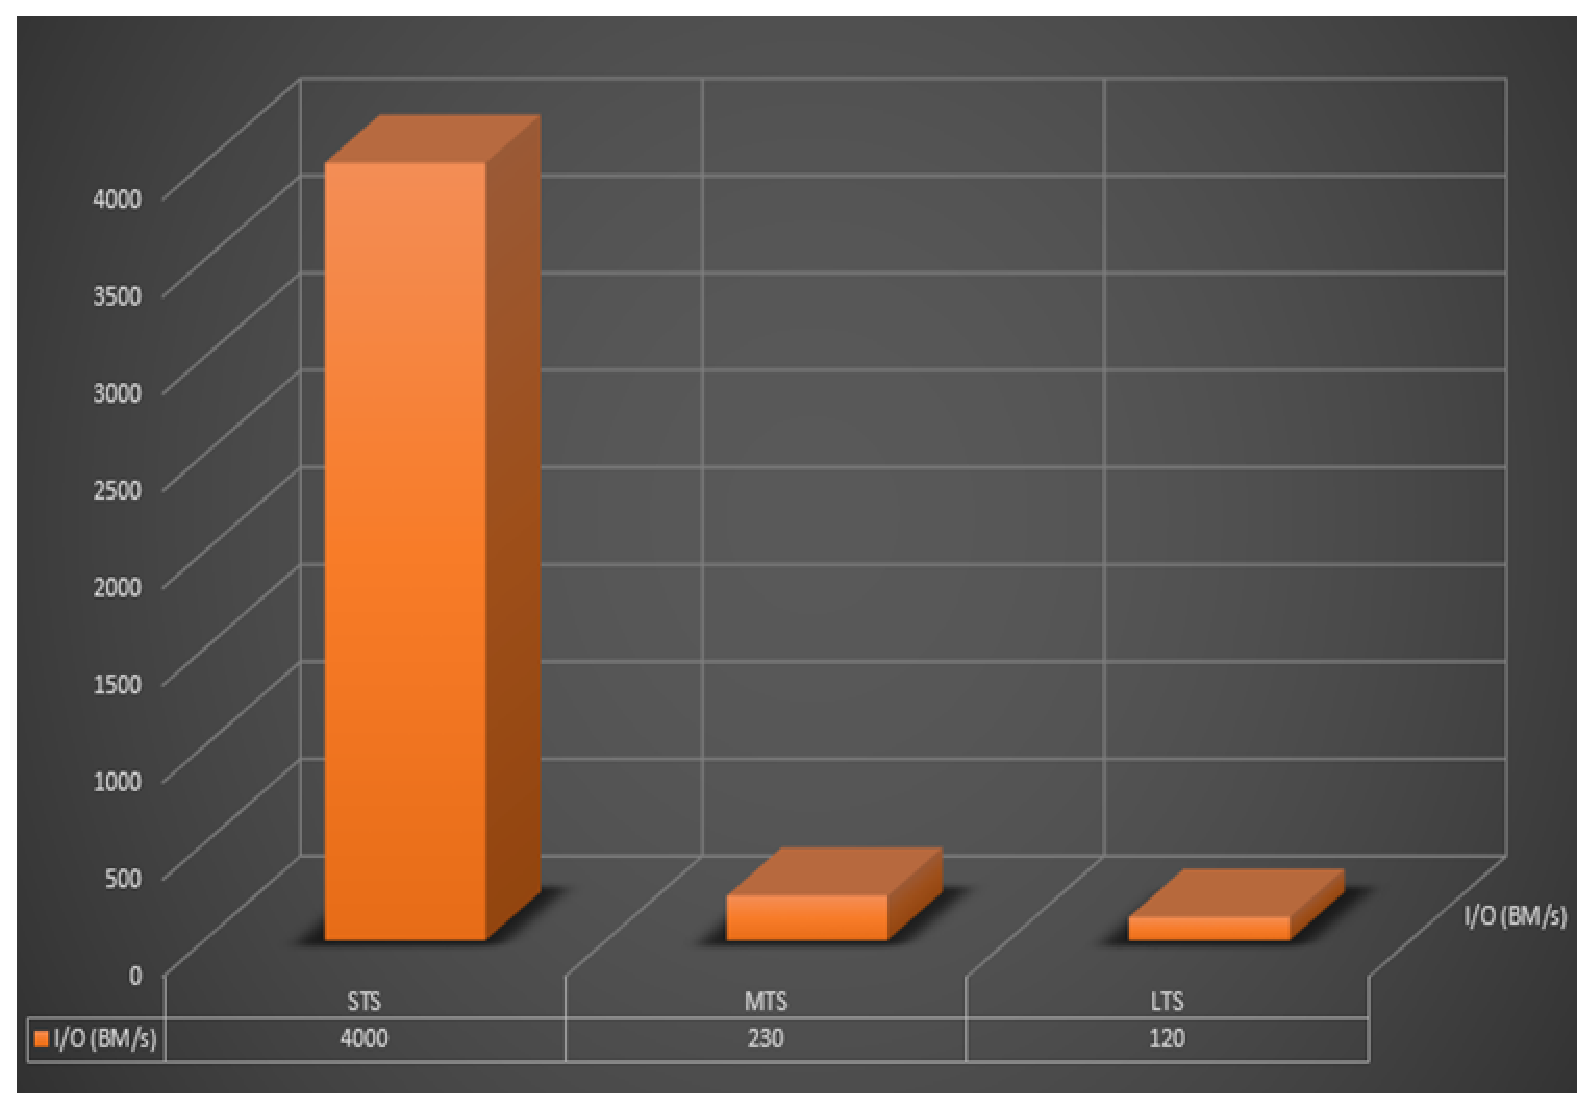
\includegraphics[width=0.65\textwidth]{./images/image-1.eps}
	\caption{File I/O Bandwidth 측정}
	\label{fig:file_bandwidth} 
\end{figure}

상위 세 스토리지 영역에서 사용하는 각각의 file system의 file I/O bandwidth를 측정하기 위하여 "dd"라는 utility를 이용하였으며 그림 \ref{fig:file_bandwidth}과 같은 결과를 얻었다. 그림 \ref{fig:file_bandwidth}에서와 같의 STS 영역의 RAM file system에 대한 file I/O bandwidth는 약 4GBytes/sec로 일반 MTS 영역의 ext4 file system과 비교하여 17배의 성능을 보이며, LTS의 gluster file system과 비교하여 33배 높은 성능을 보인다. 이는 classic channel archiver가 SATA disk 7.2k rpm에서 60,000 samples/sec 저장 능력을 보이는 것과 비교하여 산술적으로 약 1,000,000 samples/sec 저장 능력을 보일 수 있다고 판단된다. 이는 archiver appliance가 네트워크가 bandwidth가 허락하는 한도내에서 상당히 많은 EPICS PV 데이터 저장 능력을 보일 수 있다는 결론이다. 물론, 이런 가정은 memory와 disk를 mapping 시킬수 있는 가용 RAM 영역이 허락되는 범위내에서 가능하다는 전제 조건이 있다. 또한 흥미로운 부분 중 gluster file system 이다. gluster file system은 네트워크 media를 통한 네트워크 파일 시스템임에도 불구하고 NFS file system에 비하여 안정성 및 가용 bandwidth에서 우수성을 보이고 있다. 이는 네트워크 bandwidth를 10Gbps 급으로 사용한다면 local disk file system 이상의 성능을 보일 것으로 생각된다.


\section{I/O 성능 시험}
각 스토리지 영역의 bandwidth 측정 이외에도 여러 file I/O에 대한 benchmark를 위하여 IOZone\cite{iozone}이라는 benchmark tool을 활용하였다. 그림 \ref{fig:file_performance}는 각 세 영역에서 보이는 file I/O의 성능을 보여준다.

\begin{figure}[h!]
	\centering
	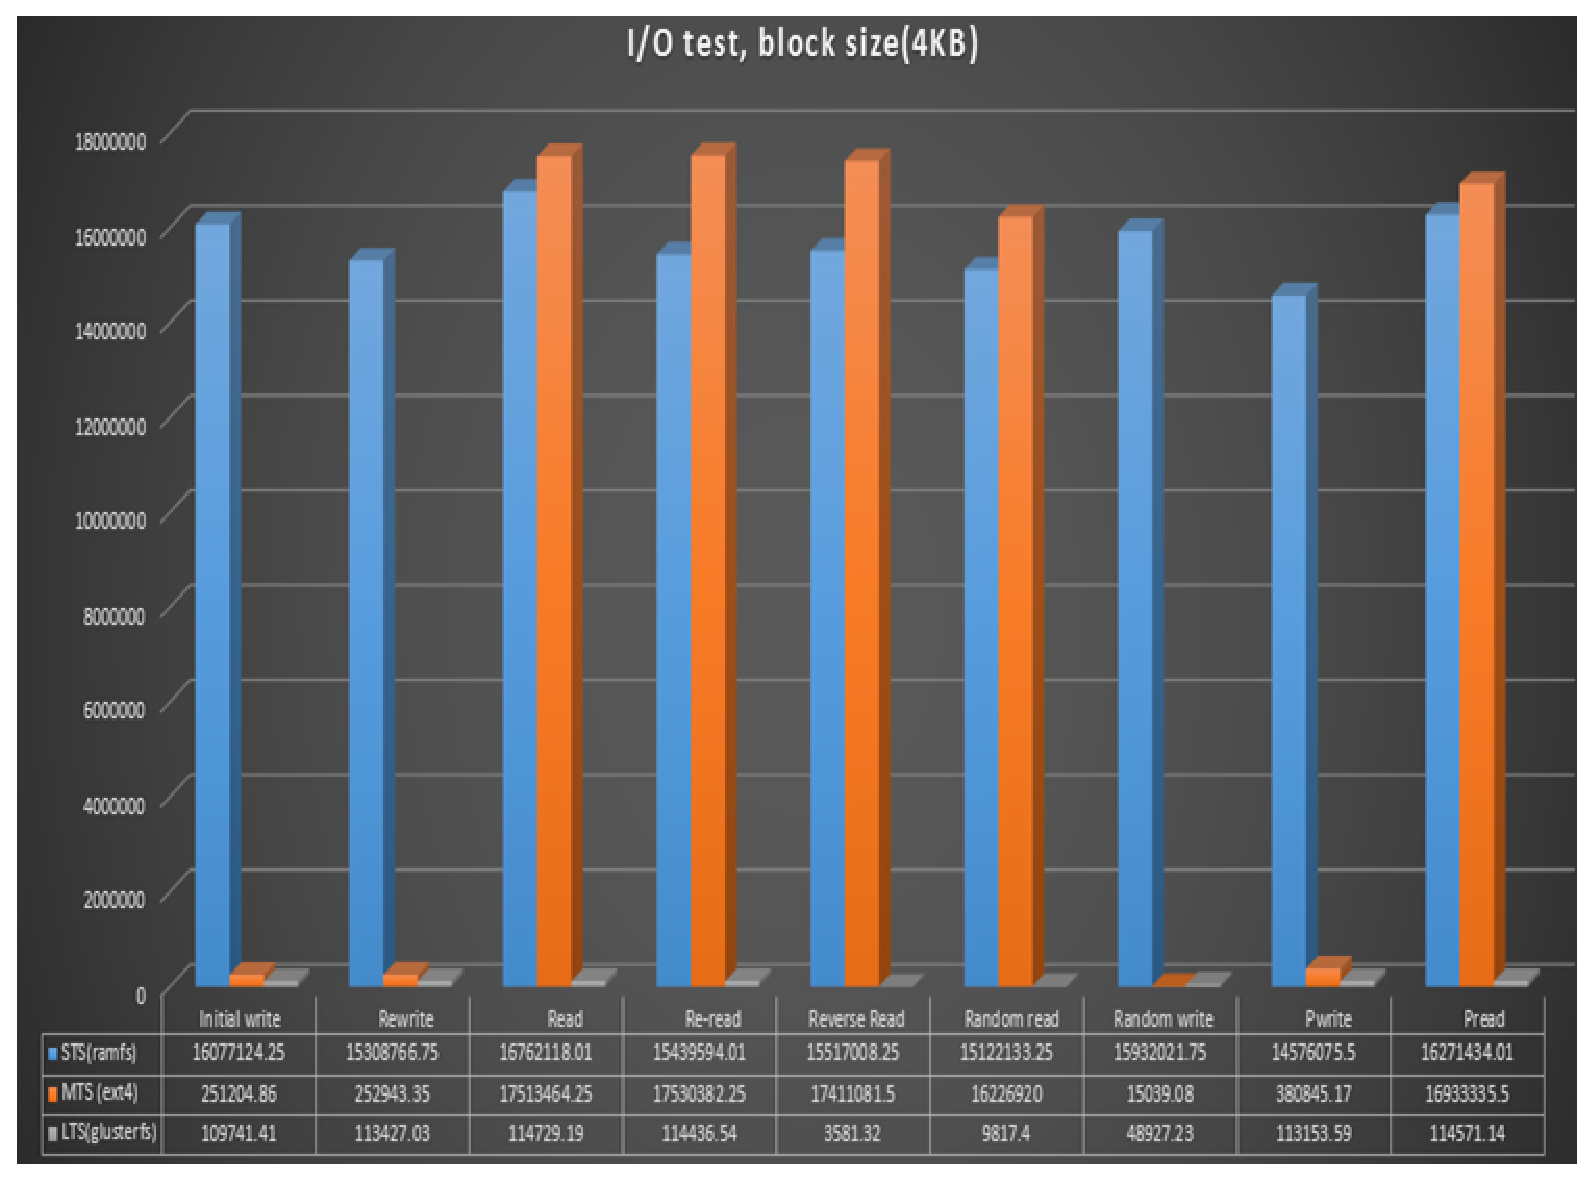
\includegraphics[width=0.75\textwidth]{./images/image-2.eps}
	\caption{File I/O 성능 측정}
	\label{fig:file_performance} 
\end{figure}

아래와 같은 test 환경으로 세 영역에서 IOZone을 실행하여 표 \ref{table:io_performance}와 같은 결과를 얻었다.

\begin{itemize}
	\item Intel Core i7-4770 CPU 3.4GHz, Quad-core 2 CPUs(8cores)
	\item Read/Write 데이터 블럭 사이즈: 4Kbytes, Channel Access의 크기와 유사한 크기
	\item 5 Cores 사용
\end{itemize}

모든 I/O 성능 시험에서 STS(ramfs) 영역이 월등히 높은 수치를 보이며, MTS (ext4)의 경우에는 데이터 write I/O에 비해 read 성능이 훨씬 좋은 결과가 나온 것을 알 수 있었다.

\begin{table}[h!]
\begin{center}
		\begin{tabular} {c|c|c|c|c|c|c|c} \hline \hline
			\cline{2-8}
			& write & rewrite & read & reread & Revread & Ranread & Ranwrite \\ \hline\hline
			STS(ramfs)  & 16077124 & 15308766 & \tiny16762118 & 15439594 & 15517008 & 15122133 & 15932021 \\ \hline\hline
			MTS(ext4)   & 251204 & 252943 & 17513464 & 17530382 & 1741108 & 16226920 & 15039  \\ \hline\hline
			LTS(glusterfs) & 109741 & 113427 & 114729 & 114436 & 3581 & 9817 & 48927  \\ \hline\hline
		\end{tabular}
		\caption{  File IO 성능 분석 }
		\label{table:io_performance} 
\end{center}
\end {table} 

\section{결과}
Appliance single 노드의 설치 및 설정, 그리고 single 노드 각 스토리지 영역별 file 성능 검증을 통하여 향 후 EPICS data 저장 시스템에 대한 필요사항 및 설계 개념을 파악하였다. 또한, single appliance 노드에 대한 파일 I/O의 성능 측정 및 임의의 EPICS Soft IOC를 생성하여 single appliance를 운영하여 아래와 같은 결과를 얻을 수 있었다.

\begin{itemize}
	\item 스토리지 영역별 file system 성능 확인
	\item 스토리지 영역별 file I/O 성능 확인
	\item 100개의 PVs의 10Hz(10 samples/sec) 를 생성하여 손실없는 데이터 저장.
	\item index file을 사용하지 않고 EPICS CA 데이터 저장 및 추출
	\item 기존 channel archiver와 비교하여 데이터 저장 볼륨 절약
	\item 단순 파일을 복사를 통하여 데이터 추출 가능
\end{itemize}

\clearpage

\chapter{향후 과제}
Single appliance 노드의 설치구성, 내용파악 및 운영을 통하여 RAON control system의 EPICS data archiving system에 대한 아래와 같은 향후 과제와 목표를 통하여 RAON accelerator 운영에 필요한 데이터 저장 시스템을 손실 없이 안정적이게 운영하여야 하겠다.

\section{Multiple Archiver Appliance 설치 구성 및 성능 시험}
\begin{itemize}
	\item Multiple appliance 노드 상에서의 환경 구성
	\item 계층적 스토리지 영역에 대한 설계(STS, MTS, LTS)
	\item LTS (Long Term Storage) 시스템에 대한 설계 및 정책(데이터 백업)
	\item Apache load balancer를 통한 대량의 데이터 획득에 대한 성능 시험 검증
	
\end{itemize}

\section{최종 구성 목표}   
\begin{itemize}
	\item RAON accelerator 운영을 위한 손실 없는 데이터 저장 시스템 구축
	\item 24시간 연속적인 무중단 데이터 서비스(Redundancy, High availability)
	\item 대량의 데이터에 대한 빠른 응답성 확보
\end{itemize}

\clearpage

\bibliographystyle{unsrtnat}
\bibliography{./refs}

\clearpage

\begin{center}
\label{appx:a}\LARGE\textbf{APPENDIX A}
\end{center}

\begin{lstlisting}[style=termstyle]
#!/bin/bash

echo "This script runs thru a typical install scenario for a single machine"
echo "You can use this to create a standard multi-instance (one Tomcat for ear WAR) tomcat deployment in a multi machine cluster by setting the ARCHAPPL_APPLIANCES and the ARCHAPPL_MYIDENTITY"
echo "For installations in a cluster, please do create a valid appliances.xml and export ARCHAPPL_APPLIANCES and ARCHAPPL_MYIDENTITY"

export SCRIPTS_DIR=`dirname $0`

if [[ ! -f ${SCRIPTS_DIR}/deployMultipleTomcats.py ]]
then
echo "Unable to determine location of this script"
exit 1
fi

if [[ ! -f ${SCRIPTS_DIR}/../mgmt.war ]]
then
echo "We need to run the script in the extracted tar.gz folder. Cannot find the mgmt.war"
exit 1
fi

echo "JAVA HOME -->"
echo ${JAVA_HOME}
echo "<--"

if [[ -z ${JAVA_HOME} ]]
then
echo "Please set JAVA_HOME to point to a 1.7 JDK"
exit 1
fi

if [[ ! -f  ${JAVA_HOME}/include/linux/jni_md.h ]]
then
echo "Missing the include/jni.md.h file in ${JAVA_HOME}. Please set JAVA_HOME to point to a 1.7 JDK (not a JRE)"
exit 1
fi

export PATH=${JAVA_HOME}/bin:${PATH}

java -version 2>&1 | grep 'version "1.7'
if (( ( $? != 0 ) ))
then
echo "Cannot find the string 1.7 in java -version. Please set JAVA_HOME to point to a 1.7 JDK"
exit 1
fi


MSG="Pick a folder (preferably empty) where you'd like to create the Tomcat instances."
echo $MSG
export DEPLOY_DIR=$(zenity  --title "$MSG" --directory --file-selection)
echo "Setting DEPLOY_DIR to ${DEPLOY_DIR}"
if [[ ! -d ${DEPLOY_DIR} ]]
then
MSG="${DEPLOY_DIR} does not seem to be a folder"
echo ${MSG}
zenity --text="${MSG}" --error
exit 1
fi

MSG="Where's the Tomcat distribution (tar.gz)?"
echo $MSG
TOMCAT_DISTRIBUTION=$(zenity  --title "$MSG" --file-selection)

if [[ ! -f ${TOMCAT_DISTRIBUTION} ]]
then
MSG="${TOMCAT_DISTRIBUTION} does not seem to be a valid file"
echo ${MSG}
zenity --text="${MSG}" --error
exit 1
fi

tar -C ${DEPLOY_DIR} -zxf  ${TOMCAT_DISTRIBUTION}

pushd ${DEPLOY_DIR}
TOMCAT_VERSION_FOLDER=`ls -d apache-tomca* | head -1`
popd

export TOMCAT_HOME=${DEPLOY_DIR}/${TOMCAT_VERSION_FOLDER}
echo "Setting TOMCAT_HOME to ${TOMCAT_HOME}"

if [[ ! -f ${TOMCAT_HOME}/conf/server.xml ]]
then
MSG="${TOMCAT_HOME} is missing the conf/server.xml file. Was ${TOMCAT_DISTRIBUTION} a valid Tomcat tar.gz?"
echo ${MSG}
zenity --text="${MSG}" --error
exit 1
fi

# Copy over the mysql client jar and create a logj.properties file.
cat > ${TOMCAT_HOME}/lib/log4j.properties <<EOF
# Set root logger level and its only appender to A1.
log4j.rootLogger=ERROR, A1
log4j.logger.config.org.epics.archiverappliance=INFO
log4j.logger.org.apache.http=ERROR


# A1 is set to be a DailyRollingFileAppender
log4j.appender.A1=org.apache.log4j.DailyRollingFileAppender
log4j.appender.A1.File=arch.log
log4j.appender.A1.DatePattern='.'yyyy-MM-dd


# A1 uses PatternLayout.
log4j.appender.A1.layout=org.apache.log4j.PatternLayout
log4j.appender.A1.layout.ConversionPattern=%-4r [%t] %-5p %c %x - %m%n
EOF

# Build the Apache Commons Daemon that ships with Tomcat
pushd ${TOMCAT_HOME}/bin
tar zxf commons-daemon-native.tar.gz
COMMONS_DAEMON_VERSION_FOLDER=`ls -d commons-daemon-*-native-src | head -1`
popd

pushd ${TOMCAT_HOME}/bin/${COMMONS_DAEMON_VERSION_FOLDER}/unix
./configure
make
if [[ ! -f jsvc ]]
then
MSG="Cannot seem to build Apache Commons demon in ${TOMCAT_HOME}/bin/${COMMONS_DAEMON_VERSION_FOLDER}/unix"
echo ${MSG}
zenity --text="${MSG}" --error
exit 1
fi
popd

cp ${TOMCAT_HOME}/bin/${COMMONS_DAEMON_VERSION_FOLDER}/unix/jsvc ${TOMCAT_HOME}/bin


MSG="Where's the mysql client jar? - this is named something like mysql-connector-java-5.1.21-bin.jar."
echo $MSG
MYSQL_CLIENT_JAR=$(zenity  --title "$MSG" --file-selection)

if [[ ! -f ${MYSQL_CLIENT_JAR} ]]
then
MSG="${MYSQL_CLIENT_JAR} does not seem to be a valid file"
echo ${MSG}
zenity --text="${MSG}" --error
exit 1
fi

cp ${MYSQL_CLIENT_JAR} ${TOMCAT_HOME}/lib
echo "Done copying the mysql client library to ${TOMCAT_HOME}/lib"

if [[ -z ${ARCHAPPL_APPLIANCES} ]]
then
MSG="I see you have not defined the ARCHAPPL_APPLIANCES environment variable. If we proceed, I'll automatically generate one in ${DEPLOY_DIR}. Should we proceed?"
echo ${MSG}
zenity --text="${MSG}" --question
if [[ $? == 0 ]] ; then
FQ_HOSTNAME=`hostname -f`
# Create an appliances.xml file and set up this appliance's identity.
cat > ${DEPLOY_DIR}/appliances.xml <<EOF
<appliances>
<appliance>
<identity>appliance0</identity>
<cluster_inetport>${FQ_HOSTNAME}:16670</cluster_inetport>
<mgmt_url>http://${FQ_HOSTNAME}:17665/mgmt/bpl</mgmt_url>
<engine_url>http://${FQ_HOSTNAME}:17666/engine/bpl</engine_url>
<etl_url>http://${FQ_HOSTNAME}:17667/etl/bpl</etl_url>
<retrieval_url>http://localhost:17668/retrieval/bpl</retrieval_url>
<data_retrieval_url>http://${FQ_HOSTNAME}:17668/retrieval</data_retrieval_url>
</appliance>
</appliances>
EOF

export ARCHAPPL_APPLIANCES=${DEPLOY_DIR}/appliances.xml
export ARCHAPPL_MYIDENTITY=appliance0
else
MSG="Please set your ARCHAPPL_APPLIANCES and ARCHAPPL_MYIDENTITY and rerun this script"
echo ${MSG}
zenity --text="${MSG}" --info
exit 1
fi
else
if [[ -z ${ARCHAPPL_MYIDENTITY} ]]
then
MSG="ARCHAPPL_APPLIANCES was defined but ARCHAPPL_MYIDENTITY was not defined. We need both of these to be defined."
echo ${MSG}
zenity --text="${MSG}" --error
exit 1
fi
fi

if [[ ! -f ${ARCHAPPL_APPLIANCES} ]]
then
MSG="${ARCHAPPL_APPLIANCES} does not seem to be a valid file."
echo ${MSG}
zenity --text="${MSG}" --error
exit 1
fi

echo "Calling ${SCRIPTS_DIR}/deployMultipleTomcats.py ${DEPLOY_DIR}"
${SCRIPTS_DIR}/deployMultipleTomcats.py ${DEPLOY_DIR}

if [[ ! -d ${DEPLOY_DIR}/mgmt/webapps ]]
then
MSG="After calling deployMultipleTomcats.py to create the tomcats for the components, we did not find the mgmt ui. One reason for this is a mismatch between the appliance identity ${ARCHAPPL_MYIDENTITY} and your appliances file at ${ARCHAPPL_APPLIANCES}. Please make that the appliance information for ${ARCHAPPL_MYIDENTITY} in ${ARCHAPPL_APPLIANCES} is correct."
echo ${MSG}
zenity --text="${MSG}" --error
exit 1	
fi

if [[ -z `which mysql` ]]
then
MSG="Unable to execute the mysql client. Is it in the PATH?"
echo ${MSG}
zenity --text="${MSG}" --error
exit 1
fi

MSG="Please enter a MySQL Connection string to an existing database like so"
DEFAULT_MYSQL_CONNECTION_STRING="--user=archappl --password=archappl --database=archappl"
echo $MSG
export MYSQL_CONNECTION_STRING=$(zenity --entry --width=800 --text="$MSG" --entry-text="${DEFAULT_MYSQL_CONNECTION_STRING}")
echo "Setting MYSQL_CONNECTION_STRING to ${MYSQL_CONNECTION_STRING}"

# Use a SHOW DATABASES command to see if the connection string is valid
let numtries=5
mysql ${MYSQL_CONNECTION_STRING} -e "SHOW DATABASES" | grep information_schema 
while (( $? && ( ${numtries} > 1) ))
do
let numtries=numtries-1
MSG="MySQL connection string ${MYSQL_CONNECTION_STRING} does not seem to be a valid connection string"
echo ${MSG}
zenity --text="${MSG}" --error
if (( ( ${numtries} <= 1 )  ))
then
# We've tried a few times; must be a bug in the script.
exit 1
fi

MSG="Please enter a MySQL Connection string like so"
DEFAULT_MYSQL_CONNECTION_STRING = ${MYSQL_CONNECTION_STRING}
echo $MSG
export MYSQL_CONNECTION_STRING=$(zenity --entry --width=800 --text="$MSG" --entry-text="${DEFAULT_MYSQL_CONNECTION_STRING}")
echo "Setting MYSQL_CONNECTION_STRING to ${MYSQL_CONNECTION_STRING}"

mysql ${MYSQL_CONNECTION_STRING} -e "SHOW DATABASES" | grep information_schema
done

# If we are here, the MYSQL_CONNECTION_STRING is valid.
# Let's check to see if the tables exist.
mysql ${MYSQL_CONNECTION_STRING} -e "SHOW TABLES" | grep PVTypeInfo
if (( ( $? != 0 ) ))
then
MSG="I do not see the PVTypeInfo table in ${MYSQL_CONNECTION_STRING}? Should we go ahead and create the tables? This step will delete any old data that you have."
echo ${MSG}
zenity --text="${MSG}" --question
if [[ $? == 0 ]] ; then
echo "Creating tables in ${MYSQL_CONNECTION_STRING}"
mysql ${MYSQL_CONNECTION_STRING} < ${SCRIPTS_DIR}/archappl_mysql.sql

mysql ${MYSQL_CONNECTION_STRING} -e "SHOW TABLES" | grep PVTypeInfo
if (( ( $? != 0 ) ))
then
MSG="Cannot create the MySQL tables. Do you have the right permissions?"
echo ${MSG}
zenity --text="${MSG}" --error
exit 1
fi
else
echo "Skipping creating MySQL tables."
fi
else 
MSG="The EPICS archiver appliance tables already exist in the schema accessed by using ${MYSQL_CONNECTION_STRING}"
echo ${MSG}
zenity --text="${MSG}" --info	
fi


# Temporarily set TOMCAT_HOME to the mgmt webapp.
TOMCAT_HOME=${DEPLOY_DIR}/mgmt
echo "Setting TOMCAT_HOME to the mgmt webapp in ${TOMCAT_HOME}"

# Add the connection pool to the context.xml file
${SCRIPTS_DIR}/addMysqlConnPool.py

# Restore TOMCAT_HOME
TOMCAT_HOME=${DEPLOY_DIR}/${TOMCAT_VERSION_FOLDER}
echo "Setting TOMCAT_HOME to ${TOMCAT_HOME}"

# Generate the deployRelease.sh script
cat > ${DEPLOY_DIR}/deployRelease.sh <<EOF
#!/bin/bash

# This script deploys a new build onto the EPICS archiver appliance installation at ${DEPLOY_DIR}
# Call this script with the folder that contains the expanded tar.gz; that is, the folder that contains the various WAR files

export JAVA_HOME=${JAVA_HOME}
export PATH=\${JAVA_HOME}/bin:\${PATH}
export TOMCAT_HOME=${TOMCAT_HOME}
export CATALINA_HOME=${TOMCAT_HOME}
export DEPLOY_DIR=${DEPLOY_DIR}

if [[ \$# -eq 0 ]]
then
echo "You need to call deployRelease.sh with the folder containing the mgmt and other war files."
exit 1
fi

WARSRC_DIR=\${1}

if [[ ! -f \${WARSRC_DIR}/mgmt.war ]]
then
echo "You need to call deployRelease.sh with the folder containing the mgmt and other war files. The folder \${WARSRC_DIR} does not seem to have a mgmt.war."
exit 1
fi

echo "Deploying a new release from \${WARSRC_DIR} onto \${DEPLOY_DIR}"
pushd \${DEPLOY_DIR}/mgmt/webapps && rm -rf mgmt*; cp \${WARSRC_DIR}/mgmt.war .; mkdir mgmt; cd mgmt; jar xf ../mgmt.war; popd; 
pushd \${DEPLOY_DIR}/engine/webapps && rm -rf engine*; cp \${WARSRC_DIR}/engine.war .; popd; 
pushd \${DEPLOY_DIR}/etl/webapps && rm -rf etl*; cp \${WARSRC_DIR}/etl.war .; popd; 
pushd \${DEPLOY_DIR}/retrieval/webapps && rm -rf retrieval*; cp \${WARSRC_DIR}/retrieval.war .; popd;
echo "Done deploying a new release from \${WARSRC_DIR} onto \${DEPLOY_DIR}"

# Post installation steps for changing look and feel etc.
if [[ -f \${WARSRC_DIR}/site_specific_content/template_changes.html ]]
then
echo "Modifying static content to cater to site specific information"
java -cp \${DEPLOY_DIR}/mgmt/webapps/mgmt/WEB-INF/classes org.epics.archiverappliance.mgmt.bpl.SyncStaticContentHeadersFooters \${WARSRC_DIR}/site_specific_content/template_changes.html \${DEPLOY_DIR}/mgmt/webapps/mgmt/ui
fi

if [[ -d \${WARSRC_DIR}/site_specific_content/img ]]
then
echo "Replacing site specific images"
cp -R \${WARSRC_DIR}/site_specific_content/img/* \${DEPLOY_DIR}/mgmt/webapps/mgmt/ui/comm/img/
fi


EOF

chmod +x ${DEPLOY_DIR}/deployRelease.sh

# Call deployRelease to deploy the WAR files.
WARSRC_DIR=`python -c "import os; print os.path.abspath('${SCRIPTS_DIR}/..')"`
echo "Calling deploy release with ${DEPLOY_DIR}/deployRelease.sh ${WARSRC_DIR}"
${DEPLOY_DIR}/deployRelease.sh ${WARSRC_DIR}

if [[ ! -f ${DEPLOY_DIR}/mgmt/webapps/mgmt/ui/index.html ]]
then
MSG="After deploying the release, cannot find a required file. The deployment did not succeed."
echo ${MSG}
zenity --text="${MSG}" --error
exit 1	
fi

cat ${SCRIPTS_DIR}/sampleStartup.sh \
| sed -e "s;export JAVA_HOME=/opt/local/java/latest;export JAVA_HOME=${JAVA_HOME};g" \
| sed -e "s;export TOMCAT_HOME=/opt/local/tomcat;export TOMCAT_HOME=${TOMCAT_HOME};g" \
| sed -e "s;export ARCHAPPL_DEPLOY_DIR=/opt/local/archappl;export ARCHAPPL_DEPLOY_DIR=${DEPLOY_DIR};g" \
| sed -e "s;export ARCHAPPL_APPLIANCES=/nfs/archiver/appliances.xml;export ARCHAPPL_APPLIANCES=${ARCHAPPL_APPLIANCES};g" \
| sed -e "s;export ARCHAPPL_MYIDENTITY=\"appliance0\";export ARCHAPPL_MYIDENTITY=\"${ARCHAPPL_MYIDENTITY}\";g" \
> ${DEPLOY_DIR}/sampleStartup.sh

MSG="Do you have a site specific policies.py file?"
echo ${MSG}
zenity --text="${MSG}" --question
if [[ $? == 0 ]]
then
MSG="Where's your site specific policies.py file?"
echo $MSG
SITE_SPECIFIC_POLICIES_FILE=$(zenity  --title "$MSG" --file-selection)

if [[ ! -f ${SITE_SPECIFIC_POLICIES_FILE} ]]
then
MSG="${SITE_SPECIFIC_POLICIES_FILE} does not seem to be a valid file"
echo ${MSG}
zenity --text="${MSG}" --error
exit 1
fi

echo "Setting ARCHAPPL_POLICIES to ${SITE_SPECIFIC_POLICIES_FILE}"
cat ${DEPLOY_DIR}/sampleStartup.sh \
| sed -e "s;# export ARCHAPPL_POLICIES=/nfs/epics/archiver/production_policies.py;export ARCHAPPL_POLICIES=${SITE_SPECIFIC_POLICIES_FILE};g" \
> ${DEPLOY_DIR}/sampleStartup.sh.withpolicies

mv -f ${DEPLOY_DIR}/sampleStartup.sh.withpolicies ${DEPLOY_DIR}/sampleStartup.sh
fi

chmod +x ${DEPLOY_DIR}/sampleStartup.sh

MSG="Done with the installation. Please use ${DEPLOY_DIR}/sampleStartup.sh to start and stop the appliance and ${DEPLOY_DIR}/deployRelease.sh to deploy a new release." 
echo ${MSG}
zenity --text="${MSG}" --info	
\end{lstlisting}
\begin{center}
\label{appx:b}\LARGE\textbf{APPENDIX B}
\end{center}
\begin{lstlisting}[style=termstyle]
#!/bin/bash

# Sample startup script for the archiver appliance
# Please change the various environment variables to suit your environment.

# We assume that we inherit the EPICS environment variables from something that calls this script
# However, if this is a init.d startup script, this is not going to be the case and we'll need to add them here.
# This includes setting up the LD_LIBRARY_PATH to include the JCA .so file.
source /opt/local/setEPICSEnv.sh

export JAVA_HOME=/opt/local/java/latest
export PATH=${JAVA_HOME}/bin:${PATH}
# We use a lot of memory; so be generous with the heap. 
export JAVA_OPTS="-XX:MaxPermSize=128M -XX:+UseG1GC -Xmx4G -Xms4G -ea"

# Set up Tomcat home
export TOMCAT_HOME=/opt/local/tomcat

# Set up the root folder of the individual Tomcat instances.
export ARCHAPPL_DEPLOY_DIR=/opt/local/archappl

# Set appliance.xml and the identity of this appliance
export ARCHAPPL_APPLIANCES=/nfs/archiver/appliances.xml
export ARCHAPPL_MYIDENTITY="appliance0"

# If you have your own policies file, please change this line.
# export ARCHAPPL_POLICIES=/nfs/epics/archiver/production_policies.py

# Set the location of short term and long term stores; this is necessary only if your policy demands it
export ARCHAPPL_SHORT_TERM_FOLDER=/arch/sts/ArchiverStore
export ARCHAPPL_MEDIUM_TERM_FOLDER=/arch/mts/ArchiverStore
export ARCHAPPL_LONG_TERM_FOLDER=/arch/lts/ArchiverStore

if [[ ! -d ${TOMCAT_HOME} ]]
then
echo "Unable to determine the source of the tomcat distribution"
exit 1
fi

if [[ ! -f ${ARCHAPPL_APPLIANCES} ]]
then
echo "Unable to find appliances.xml at ${ARCHAPPL_APPLIANCES}"
exit 1
fi

# Enable core dumps in case the JVM fails
ulimit -c unlimited




function startTomcatAtLocation() { 
if [ -z "$1" ]; then echo "startTomcatAtLocation called without any arguments"; exit 1; fi
export CATALINA_HOME=$TOMCAT_HOME
export CATALINA_BASE=$1
echo "Starting tomcat at location ${CATALINA_BASE}"

ARCH=`uname -m`
if [[ $ARCH == 'x86_64' || $ARCH == 'amd64' ]]
then
echo "Using 64 bit versions of libraries"
export LD_LIBRARY_PATH=${CATALINA_BASE}/webapps/engine/WEB-INF/lib/native/linux-x86_64:${LD_LIBRARY_PATH}
else
echo "Using 32 bit versions of libraries"
export LD_LIBRARY_PATH=${CATALINA_BASE}/webapps/engine/WEB-INF/lib/native/linux-x86:${LD_LIBRARY_PATH}
fi

pushd ${CATALINA_BASE}/logs
${CATALINA_HOME}/bin/jsvc \
-server \
-cp ${CATALINA_HOME}/bin/bootstrap.jar:${CATALINA_HOME}/bin/tomcat-juli.jar \
${JAVA_OPTS} \
-Dcatalina.base=${CATALINA_BASE} \
-Dcatalina.home=${CATALINA_HOME} \
-outfile ${CATALINA_BASE}/logs/catalina.out \
-errfile ${CATALINA_BASE}/logs/catalina.err \
-pidfile ${CATALINA_BASE}/pid \
org.apache.catalina.startup.Bootstrap start
popd
}

function stopTomcatAtLocation() { 
if [ -z "$1" ]; then echo "stopTomcatAtLocation called without any arguments"; exit 1; fi
export CATALINA_HOME=$TOMCAT_HOME
export CATALINA_BASE=$1
echo "Stopping tomcat at location ${CATALINA_BASE}"
pushd ${CATALINA_BASE}/logs
${CATALINA_HOME}/bin/jsvc \
-server \
-cp ${CATALINA_HOME}/bin/bootstrap.jar:${CATALINA_HOME}/bin/tomcat-juli.jar \
${JAVA_OPTS} \
-Dcatalina.base=${CATALINA_BASE} \
-Dcatalina.home=${CATALINA_HOME} \
-outfile ${CATALINA_BASE}/logs/catalina.out \
-errfile ${CATALINA_BASE}/logs/catalina.err \
-pidfile ${CATALINA_BASE}/pid \
-stop \
org.apache.catalina.startup.Bootstrap 
popd
}

function stop() { 
stopTomcatAtLocation ${ARCHAPPL_DEPLOY_DIR}/engine
stopTomcatAtLocation ${ARCHAPPL_DEPLOY_DIR}/retrieval
stopTomcatAtLocation ${ARCHAPPL_DEPLOY_DIR}/etl
stopTomcatAtLocation ${ARCHAPPL_DEPLOY_DIR}/mgmt
}

function start() { 
startTomcatAtLocation ${ARCHAPPL_DEPLOY_DIR}/mgmt
startTomcatAtLocation ${ARCHAPPL_DEPLOY_DIR}/engine
startTomcatAtLocation ${ARCHAPPL_DEPLOY_DIR}/etl
startTomcatAtLocation ${ARCHAPPL_DEPLOY_DIR}/retrieval
}


# See how we were called.
case "$1" in
start)
start
;;
stop)
stop
;;
restart)
stop
start
;;
*)
echo $"Usage: $0 {start|stop|restart}"
exit 2
esac
\end{lstlisting}
\begin{center}
\label{appx:c}\LARGE\textbf{APPENDIX C}
\end{center}
\begin{lstlisting}[style=termstyle]
#!/usr/bin/env python

# This script deploys a archiver appliance build onto a appliance into four separate JVM's as per the documentation.
# The artifacts from the build are four war files that are independent of each other. 
# One can choose to deploy all of these on one JVM; however, as the archiver appliance is a fairly memory intensive application; this can adversely impact GC on the single JVM.
# Also, one does not want a large user retrieval to affect the engine or ETL.
# Therefore, there are some advantages to deploying each war file on a separate JVM.

# This script uses TOMCAT_HOME to determine the source of the Tomcat distribution.
# It then makes four subfolders in the specified folder, one each for the mgmt, engine, etl and retrieval webapps.
# It copies over the necessary content from the source into each of these subfolders and adjusts the configuration as necessary.
# It then deploys the war files into the appropriate tomcats.
# The war files are assumed to be in the parent folder; however you can use an option to override this. 

# This is the just the deployment step; you can then have individual /etc/init.d scripts (or use commons daemon) to start the four webapps.
# So your deployment script should be something like 1) Stop webapps 2) Deploy webapps using this script 3) Start webapps.

# The appliance port configuration is determined from appliances.xml as specified in the ARCHAPPL_APPLIANCES environment variable.
# The identity for this appliance is determined from the ARCHAPPL_MYIDENTITY environment variable and ise used to lookup the parameters for this appliance in appliances.xml.
# The tomcat start/stop ports are set by incrementing the port specified in the source for each of the webapps.

# To generate start and stop script use something like this
# export CATALINA_HOME=$TOMCAT_HOME
# DEPLOY_DIR=/opt/local/ArchiverAppliance/tomcats
# The stop sequences....
# export CATALINA_BASE=${DEPLOY_DIR}/mgmt; ${CATALINA_HOME}/bin/catalina.sh stop 
# export CATALINA_BASE=${DEPLOY_DIR}/engine; ${CATALINA_HOME}/bin/catalina.sh stop 
# export CATALINA_BASE=${DEPLOY_DIR}/etl; ${CATALINA_HOME}/bin/catalina.sh stop 
# export CATALINA_BASE=${DEPLOY_DIR}/retrieval; ${CATALINA_HOME}/bin/catalina.sh stop 
# The start sequences
# export CATALINA_BASE=${DEPLOY_DIR}/mgmt; ${CATALINA_HOME}/bin/catalina.sh start
# export CATALINA_BASE=${DEPLOY_DIR}/engine; ${CATALINA_HOME}/bin/catalina.sh start
# export CATALINA_BASE=${DEPLOY_DIR}/etl; ${CATALINA_HOME}/bin/catalina.sh start
# export CATALINA_BASE=${DEPLOY_DIR}/retrieval; ${CATALINA_HOME}/bin/catalina.sh start

import sys
import os
import xml.dom.minidom
import urlparse
import shutil

def deployMultipleTomcats(destFolder):
tomcatHome = os.getenv("TOMCAT_HOME")
if tomcatHome == None:
print "We determine the source Tomcat distribution using the environment variable TOMCAT_HOME which does not seem to be set."
sys.exit(1)
thisAppliance = os.getenv("ARCHAPPL_MYIDENTITY")
if thisAppliance == None:
print "We determine the identity of this appliance using the environment variable ARCHAPPL_MYIDENTITY which does not seem to be set."
sys.exit(1)
appliancesXML = os.getenv("ARCHAPPL_APPLIANCES")
if appliancesXML == None:
print "We determine the location of the appliances.xml file using the environment variable ARCHAPPL_APPLIANCES which does not seem to be set."
sys.exit(1)

print "Using\n\ttomcat installation at", tomcatHome, "\n\tto generate deployments for appliance", thisAppliance, "\n\tusing configuration info from", appliancesXML, "\n\tinto folder", destFolder

# Parse the tomcat/conf/server.xml file and determine the stop start port
# We start incrementing and use this port+1 for each of the new webapps
tomcatServerConfSrc = tomcatHome + '/conf/server.xml'
serverdom = xml.dom.minidom.parse(tomcatServerConfSrc);
serverStopStartPort = serverdom.getElementsByTagName('Server').item(0).getAttribute('port')
if int(serverStopStartPort) == 8005:
print "The start/stop port is the standard Tomcat start/stop port. Changing it to something else random - 16000"
serverStopStartPort='16000'
newServerStopStartPort = int(serverStopStartPort)+1
print 'The stop/start ports for the new instance will being at ', newServerStopStartPort

# Parse the appliances.xml and determine the ports for the HTTP listeners
appliancesXMLDOM =  xml.dom.minidom.parse(appliancesXML)
appliances = appliancesXMLDOM.getElementsByTagName('appliance')
for appliance in appliances:
identity = appliance.getElementsByTagName('identity').item(0).firstChild.data
if identity != thisAppliance:
# print "Skipping config for", appliance, " looking for ", thisAppliance
continue
httplistenerports = {}
mgmtUrl = appliance.getElementsByTagName('mgmt_url').item(0).firstChild.data
engineUrl = appliance.getElementsByTagName('engine_url').item(0).firstChild.data
etlUrl = appliance.getElementsByTagName('etl_url').item(0).firstChild.data
retrievalUrl = appliance.getElementsByTagName('retrieval_url').item(0).firstChild.data
httplistenerports['mgmt'] = urlparse.urlparse(mgmtUrl).port
httplistenerports['engine'] = urlparse.urlparse(engineUrl).port
httplistenerports['etl'] = urlparse.urlparse(etlUrl).port
httplistenerports['retrieval'] = urlparse.urlparse(retrievalUrl).port

for app in ['mgmt', 'engine', 'etl', 'retrieval']:
# Delete any existing subfolders if any and make new ones.
subFolder = destFolder + '/' + app
if os.access(subFolder, os.W_OK):
print "Removing ", subFolder
shutil.rmtree(subFolder)
print "Generating tomcat folder for ", app, " in location", subFolder
os.makedirs(subFolder)
# See http://kief.com/running-multiple-tomcat-instances-on-one-server.html for the steps we are using here.
shutil.copytree(tomcatHome + '/conf', subFolder + '/conf')
shutil.copytree(tomcatHome + '/webapps', subFolder + '/webapps')
os.makedirs(subFolder + '/logs')
os.makedirs(subFolder + '/temp')
os.makedirs(subFolder + '/work')

# print 'StopStart for', app, ' is', newServerStopStartPort, "and the HTTP listener port as determined from appliances.xml is", httplistenerports[app]
newServerDom = xml.dom.minidom.parse(subFolder + '/conf/server.xml')
newServerDom.getElementsByTagName('Server').item(0).setAttribute('port', str(newServerStopStartPort))
# Find the 'Connector' whose 'protocol' is 'HTTP/1.1'
haveSetConnector = False
for httplistenerNode in newServerDom.getElementsByTagName('Connector'):
if httplistenerNode.hasAttribute('protocol') and httplistenerNode.getAttribute('protocol') == 'HTTP/1.1':
httplistenerNode.setAttribute('port', str(httplistenerports[app]))
haveSetConnector = True
else:
print "Commenting connector with protocol ", httplistenerNode.getAttribute('protocol'), ". If you do need this connector, you should un-comment this."
comment = httplistenerNode.ownerDocument.createComment(httplistenerNode.toxml())
httplistenerNode.parentNode.replaceChild(comment, httplistenerNode)
if haveSetConnector == False:
raise AssertionError("We have not set the HTTP listener port for " + app);


with open(subFolder + '/conf/server.xml', 'w') as file: 
newServerDom.writexml(file)
newServerStopStartPort =  newServerStopStartPort+1

if __name__ == "__main__":
if len(sys.argv) < 2:
print "Usage: ", sys.argv[0], "<DeploymentFolder>"
sys.exit(1)
deployMultipleTomcats(sys.argv[1])
\end{lstlisting}

\begin{center}
\label{appx:d}\LARGE\textbf{APPENDIX D}
\end{center}

\begin{lstlisting}[style=termstyle]
#!/usr/bin/env python

# This script adds a EPICS archiver appliance MySQL connection pool to a Tomcat context.xml
# The location of context.xml is determined by the ${TOMCAT_HOME} environment variable
# The parameters for the connection pool are determined by the ${MYSQL_CONNECTION_STRING} environment variable  

import sys
import os
import xml.dom.minidom
import urlparse
import shutil

mysql_connection_string = os.getenv('MYSQL_CONNECTION_STRING')
if not mysql_connection_string:
print 'The environment variable MYSQL_CONNECTION_STRING is not defined. Please define using export MYSQL_CONNECTION_STRING="--user=archappl --password=archappl --database=archappl"'
sys.exit(1)

tomcatHome = os.getenv("TOMCAT_HOME")
if tomcatHome == None:
print "We determine the location of context.xml using the environment variable TOMCAT_HOME which does not seem to be set."
sys.exit(1)

connpoolparams = {}
for mysqlparam in mysql_connection_string.split():
paramnv = mysqlparam.split('=')
paramame = paramnv[0].replace('--', '')
paramval = paramnv[1]
connpoolparams[paramame] = paramval

if 'user' not in connpoolparams:
print 'Cannot determine the user from ", mysql_connection_string, ". Please define like so "--user=archappl --password=archappl --database=archappl"'
sys.exit(1)

if 'password' not in connpoolparams:
print 'Cannot determine the user from ", mysql_connection_string, ". Please define like so "--user=archappl --password=archappl --database=archappl"'
sys.exit(1)

if 'database' not in connpoolparams:
print 'Cannot determine the user from ", mysql_connection_string, ". Please define like so "--user=archappl --password=archappl --database=archappl"'
sys.exit(1)

user=connpoolparams['user']
pwd=connpoolparams['password']
db=connpoolparams['database']

tomcatContextXML = tomcatHome + '/conf/context.xml'
serverdom = xml.dom.minidom.parse(tomcatContextXML);
resources = serverdom.getElementsByTagName('Resource')
for resource in resources:
if resource.getAttribute('name') == 'jdbc/archappl':
print "Connection pool jdbc/archappl is already defined"
sys.exit(0)


connpool =  serverdom.createElement('Resource')
connpool.setAttribute('name',"jdbc/archappl")
connpool.setAttribute('auth',"Container")
connpool.setAttribute('type',"javax.sql.DataSource")
connpool.setAttribute('factory',"org.apache.tomcat.jdbc.pool.DataSourceFactory")
connpool.setAttribute('testWhileIdle',"true")
connpool.setAttribute('testOnBorrow',"true")
connpool.setAttribute('testOnReturn',"false")
connpool.setAttribute('validationQuery',"SELECT 1")
connpool.setAttribute('validationInterval',"30000")
connpool.setAttribute('timeBetweenEvictionRunsMillis',"30000")
connpool.setAttribute('maxActive',"10")
connpool.setAttribute('minIdle',"2")
connpool.setAttribute('maxWait',"10000")
connpool.setAttribute('initialSize',"2")
connpool.setAttribute('removeAbandonedTimeout',"60")
connpool.setAttribute('removeAbandoned',"true")
connpool.setAttribute('logAbandoned',"true")
connpool.setAttribute('minEvictableIdleTimeMillis',"30000")
connpool.setAttribute('jmxEnabled',"true")
connpool.setAttribute('driverClassName',"com.mysql.jdbc.Driver")
connpool.setAttribute('url',"jdbc:mysql://localhost:3306/" + connpoolparams['database'])
connpool.setAttribute('username',connpoolparams['user'])
connpool.setAttribute('password',connpoolparams['password'] )

serverdom.getElementsByTagName('Context')[0].appendChild(connpool)

with open(tomcatContextXML, 'w') as file: 
file.write(serverdom.toprettyxml())
\end{lstlisting}
\begin{center}
	\label{appx:e}\LARGE\textbf{APPENDIX E}
\end{center}
\begin{lstlisting}[style=termstyle]
CREATE TABLE PVTypeInfo ( 
pvName VARCHAR(255) NOT NULL PRIMARY KEY,
typeInfoJSON MEDIUMTEXT NOT NULL,
last_modified TIMESTAMP DEFAULT CURRENT_TIMESTAMP ON UPDATE CURRENT_TIMESTAMP
) ENGINE=InnoDB;

CREATE TABLE PVAliases (
pvName VARCHAR(255) NOT NULL PRIMARY KEY,
realName VARCHAR(256) NOT NULL,
last_modified TIMESTAMP DEFAULT CURRENT_TIMESTAMP ON UPDATE CURRENT_TIMESTAMP
) ENGINE=InnoDB;

CREATE TABLE ArchivePVRequests ( 
pvName VARCHAR(255) NOT NULL PRIMARY KEY,
userParams MEDIUMTEXT NOT NULL,
last_modified TIMESTAMP DEFAULT CURRENT_TIMESTAMP ON UPDATE CURRENT_TIMESTAMP
) ENGINE=InnoDB;

CREATE TABLE ExternalDataServers ( 
serverid VARCHAR(255) NOT NULL PRIMARY KEY,
serverinfo MEDIUMTEXT NOT NULL,
last_modified TIMESTAMP DEFAULT CURRENT_TIMESTAMP ON UPDATE CURRENT_TIMESTAMP
) ENGINE=InnoDB;

\end{lstlisting}
\end{document}

